\documentclass[10pt]{article}
\usepackage{zsj}

\usepackage{silence}
\WarningFilter{latex}{Marginpar on page}

\allowdisplaybreaks

\hbadness=99999


\begin{document}
\title{Topology and Geometry}
\subheader{Notes}
\author{Shangjie Zhou\orcidlink{0000-0001-9576-5011}}
\affiliation{School of Physics and Technology, Wuhan University}
\emailAdd{sjzhou@whu.edu.cn}
\abstract{\textit{Last updated on: \today}\\Source files: \url{https://github.com/spaceofzsj/Conformal-Field-Theory/releases}\\Website: \url{https://spaceofzsj.github.io/ShangjieZhou/}}

\maketitle

\section*{Introduction}
\addcontentsline{toc}{section}{\protect\numberline{}Introduction}
This notes follow the book by Nakahara\cite{Nakahara:1990th}.
\clearpage
\part{Topology}
\section{Mathematical Preliminaries}
\subsection{Maps}
\subsubsection{Definitions}
\begin{definition}[Map]
    Let $X$ and $Y$ be sets.
    A \textbf{map} (or \textbf{mapping}) $f$ is a rule by which we assign $y\in Y$ for each $x\in X$.
\end{definition}
We write
\begin{align}
    f:X\to Y.
\end{align}
If $f$ is defined by some explicit formula, we write
\begin{align}
    f:x\mapsto f(x).
\end{align}

\begin{definition}[Injective, surjective, bijective]
    If a map satisfies a certain condition it bears a special name.
    \begin{itemize}
        \item A map $f:X\to Y$ is called \textbf{injective} (or \textbf{one to one}) if $x\neq x'$implies $f(x)\neq f(x')$.
        \item A map $f:X\to Y$ is called \textbf{surjective} (or \textbf{onto}) if for each $y\in Y$ there exists at least one element $x\in X$ such that $f(x)=y$.
        \item A map $f:X\to Y$ is called \textbf{bijective} if it is both injective and surjective.
    \end{itemize}
\end{definition}
\subsubsection{Equivalence Relation and Equivalence Class}
\begin{definition}[Relation]
    A relation $R$ in a set $X$ is a subset of $X\times X$.
\end{definition}
If a point $(a,b)\in X\times X$ is in a relation $R$, then we write $aRb$.
\begin{definition}[Equivalence relation]
    An equivalence relation $\sim$ is a relation which satisfies the following requirements
    \begin{itemize}
        \item \textit{reflective}: $a\sim a$.
        \item \textit{symmetric}: If $a\sim b$, then $b\sim a$.
        \item \textit{transitive}: If $a\sim b$ and $b\sim c$, then $a\sim c$.
    \end{itemize}
\end{definition}
\subsection{Vector Spaces}
\subsubsection{Vectors and Vector Spaces}
\begin{definition}[Vector space]
    A \textbf{vector space} (or a \textbf{linear space}) $V$ over a field $K$ is a set in which two operations, addition and multiplication by an element of $K$ (called a \textbf{scalar}),
    are defined (In this notes we are mainly interested in $K=\mathbb{R}$ and $\mathbb{C}$).
    The elements of $V$ (called \textbf{vectors}) satisfy the following axioms:
    \begin{itemize}
        \item $\vb*{u}+\vb*{n}=\vb*{v}+\vb*{u}$.
        \item $(\vb*{u}+\vb*{v})+\vb*{w}=\vb*{u}+(\vb*{v}+\vb*{w})$.
        \item There exists a zero vector $\vb*{0}$ such that $\vb*{v}+\vb*{0}=\vb*{v}$.
        \item For any $\vb*{u}$, there exists $-\vb*{u}$, such that $\vb*{u}+(-\vb*{u})=0$.
        \item $c(\vb*{u}+\vb*{v})+c\vb*{u}+c\vb*{v}$.
        \item $(cd)\vb*{u}=c(d\vb*{u})$.
        \item $1 \vb*{u}=\vb*{u}$.
    \end{itemize}
    Here $\vb*{u}, \vb*{v}, \vb*{w}$ and $c,d\in K$ and $1$ is the unit element of $K$.
\end{definition}
In this note, we only consider vector spaces over $\mathbb{R}$ or $\mathbb{C}$.

\begin{definition}[Convex combination]
    If $V$ is a vector space, we call elements $\vb*{v}'$ in $V$ convex combinations of $\vb*{v}_1,\vb*{v}_2,\dots,\vb*{v}_n\in V$ if it satisfies the following form:
    \begin{equation}
        v'=\alpha_1 \vb*{v}_1+\alpha_2 \vb*{v}_2+\dots \alpha_n \vb*{v}_n
    \end{equation}
    where $\alpha_1,\alpha_2,\dots,\alpha_n$ are positive real numbers and $\sum_{i=1}^{n}\alpha_i=1$.
\end{definition}

\begin{definition}[Convex set]
    Let $V$ be a vector space and $K\subset V$.
    The set $K$ is said to be convex if any convex combination of elements in $K$ is still an element in $K$.
\end{definition}

\begin{definition}[Extreme point]
    A extreme point of a convex set $K$ is a point $x\in K$ with the property: there does not exist $y,z\in K$ and $t\in(0,1)$ such that $y\neq z$ and $x=ty+(1-t)z$.
    The set of all extreme points of $K$ is denoted by $\text{extreme}(K)$.
\end{definition}

\begin{definition}[Convex hull]
    The convex hull (or convex envelope) of a given set $X$ is defined to be the set of all convex combinations of points in $X$.
\end{definition}

\begin{definition}[Cone]
    A subset $C$ of a vector space $V$ is called a cone if for $\alpha>0$ and each $x\in C$, the element $\alpha x$ is in $C$.
\end{definition}

\begin{definition}[Convex cone]
    A cone $C$ in a vector space $V$ is called a convex cone if $C$ is convex.
\end{definition}

\subsubsection{Linear Maps, Images and Kernels}
\begin{theorem}
    If $f:V\to W$ is a linear map, then
    \begin{align}
        \dim{V}=\dim(\ker{f})+\dim(\im f).
    \end{align}
\end{theorem}
\begin{proof}
    to be added
\end{proof}

\subsubsection{Dual Vector Space}

\subsubsection{Inner Product and Adjoint}
\begin{theorem}[Toy index theorem]
    Let $V$ and $W$ be finite-dimensional vector spaces over a field $K$ and let $f:V\to W$ be a linear map.
    Then
    \begin{align}
        \dim\ker f-\dim\ker\tilde{f}=\dim V-\dim W.
    \end{align}
\end{theorem}
\begin{proof}
    to be added
\end{proof}

\subsubsection{Tensors}

\subsection{Topological Spaces}
\subsubsection{Definitions}
\begin{definition}[Topological space]
    Let $X$ be any set and $\mathcal{T}=\left\{U_i\vert i\in I\right\}$ denote a certain collection of subsets of $X$.
    The pair $(X,\mathcal{T})$ is a topological space if $\mathcal{T}$ satisfies the following requirements
    \begin{enumerate}
        \item $\emptyset,X\in\mathcal{T}$
        \item If $J$ is any (maybe infinite) subset of $I$, the family $\left\{U_j\vert j\in J\right\}$ satisfies $\cup_{j\in J}U_j\in \mathcal{T}$.
        \item If $K$ is any finite subset of $I$, the family $\left\{U_k\vert k\in K\right\}$ satisfies $\cap_{k\in K}U_k\in\mathcal{T}$.
    \end{enumerate}
    The $U_i$ are called the open sets and $\mathcal{T}$ is said to give a topology to $X$.
\end{definition}

\subsubsection{Continuous Maps}
\begin{definition}[Continuous map]
    Let $X$ and $Y$ be topological spaces.
    A map $f:X\to Y$ is continuous if the inverse image of an open set in $Y$ is an open set in $X$.
\end{definition}

\subsubsection{Neighbourhoods and Hausdorff Spaces}
\begin{definition}[Neighbourhood]
    Suppose $\mathcal{T}$ gives a topology to $X$.
    $N$ is a neighbourhood of a point $x\in X$ if $N$ is a subset of $X$ and $N$ contains some (at least one) open set $U_i$ to which $x$ belongs.
    If $N$ is also a open set in $\mathcal{T}$, then we call $N$ a open neighbourhood.
\end{definition}

\begin{definition}[Hausdorff space]
    A topological space $(X,\mathcal{T})$ is called a Hausdorff space if, for an arbitrary pair of distinct points $x,x'\in X$, there always exist neighbourhoods $U_x$ of $x$ and $U_{x'}$ of $x'$ such that $U_x\cup U_{x'}=\emptyset$.
\end{definition}

\subsubsection{Closed set}
\begin{definition}[Closed set]
    Let $(X,\mathcal{T})$ be a topological space.
    A subset of $A$ of $X$ is closed if its complement in $X$ is an open set, that is $X_A\in\mathcal{T}$.
\end{definition}

\begin{definition}[Limit point]
    Let $S$ be a subset of a topological space $X$.
    A point $x\in X$ is a limit point of $S$ if every neighbourhood of $x$ contains at lease one point of $S$ different from $x$ it self.
\end{definition}

\begin{definition}[Derived set]
    Let $(X,\mathcal{T})$ be a topological space and $S\subset X$.
    The derived set of $S$ is defined to be the set of limit points of $S$ and is often denoted by $S'$.
\end{definition}

\begin{definition}[Closure, interior and boundary]
    Let $(X,\mathcal{T})$ be a topological space and $A\subset X$.
    \begin{itemize}
        \item The closure of $A$ is defined to be $A\cup A'$ ($A'$ is the derived set) and is denoted by $\bar{A}$.
        \item The interior of $A$ is defined to be the union of all open subsets of $A$ and is denoted by $A^\circ$.
        \item The boundary $b(A)$ (also often denoted by $\partial A$) of $A$ is the complement of $A^\circ$ in $A$, that is $b(A)\equiv A-A^\circ$.
    \end{itemize}
\end{definition}

\subsubsection{Compactness}
\begin{definition}[Covering]
    Let $(X,\mathcal{T})$ be a topological space.
    A family $\left\{A_i\vert i\in I\right\}$ of subsets of $X$ is called a covering of $X$, if 
    \begin{equation}
        \bigcup_{i\in I} A_i=X.
    \end{equation}
    If all the $A_i$ are open sets of $\mathcal{T}$, then the covering is called an open covering.
\end{definition}

\begin{definition}[Compactness]
    Let $(X,\mathcal{T})$ be a topological space.
    The set $X$ is compact if, for every open covering $\left\{U_i\vert i\in I\right\}$, there exists a finite subset $J$ of $I$ such that $\left\{U_j\vert j\in J\right\}$ is also a covering of $X$.
\end{definition}

\subsection{Homeomorphisms and Topological Invariants}
\subsubsection{Homeomorphisms}
\begin{intu}
    The purpose of topology is to classify spaces.
\end{intu}

For example, in elementary geometry, the equivalence of figures is given by congruence, which turns out to be too stringent for our purpose.
In topolgy, we define two figures to be equivalent if it is possible to deform one figure into the other by \textit{continuous deformation}.
\begin{definition}[Homeomorphism]\label{homeomorphism}
    Let $X_1$ and $X_2$ be topological spaces.
    A map $f : X_{1}\to X_{2}$ is a \textbf{homeomorphism} if it is continuous and has an inverse $f^{-1}:X_{2}\to X_{1}$ which is also continuous.
    If there exists a homeomorphism between $X_1$ and $X_2$ , $X_1$ is said to be \textbf{homeomorphic} to $X_2$ and vice versa.
\end{definition}

A homeomorphism is an equivalence relation and the proof is:
\begin{proof}
    \begin{itemize}
        \item Reflectivity: simply choose $f=\text{id}_X$.
        \item Symmetry: by definition, if $f : X_1 \to X_2$ is a homeomorphism, so is $f^{-1} : X_2 \to X_1$. (Using $(f^{-1})^{-1}=f$)
        \item Transitivity: if $f : X_1 \to X_2$ and $g : X_2 \to X_3$ are homeomorphisms, so is $g\circ f : X_1\rightarrow X_3$.
    \end{itemize}
\end{proof}

Intuitively speaking, two topological spaces are homeomorphic to each other if we can deform one into the other continuously, that is, without tearing them apart or pasting.
\begin{example}
    An open disc $D^2= \left\{ (x,y)\in\mathbb{R}^{2}|x^2+y^2<1 \right\}$ is homeomorphic to $\mathbb{R}^2$ when we choose
    \begin{align}
        f(x,y)=\left(\frac{x}{\sqrt{1-x^2-y^2}},\frac{y}{1-x^2-y^2}\right)
    \end{align}
\end{example}

\subsubsection{Topological Invariants}
\textbf{Topological invariants} are quantities to characterize equivalence clsses of homeomorphism.

If two spaces are homeomorphic to each other,they have the same "topological invariants".
And if two spaces have different "topological invariants",they are not homeomorphic to each other.

\subsubsection{Homotomy type}
\begin{intu}
    The condition of homeomorphism is too restrict, we will see it would be useful to define a new equivalent class, namely of the \textit{same homotopy type}.
\end{intu}

Just relax the condition in \cref{homeomorphism} so that the continuous functions $f$ and $g$ need not have inverses.

\subsubsection{Euler Characteristic: An Example}
In this section, We focus on $\mathbb{R}^3$.
\begin{definition}[Euler characteristic]
    Let $X$ be a subset of $\mathbb{R}^3$, which is homeomorphic to a polyderon $K$.
    Then the \textbf{Euler characteristic} $\chi(X)$ of $X$ is defined by
    \begin{align}
        \chi(X)= & (\text{number of verticies in}\ K)-(\text{number of edges in}\ K)\notag \\
                 & +(\text{number of faces in}\ K)
    \end{align}
\end{definition}

\begin{theorem}[Poincar{\'e}-Alexander]
    The Euler characteristic $\chi(X)$ is idependent of the polyhedron $K$ as long as $K$ is homeomorphic to $X$.
\end{theorem}

The \textit{connected sum} $X \sharp Y$ of two surfaces $X$ and $Y$ is a surface obtained by removing a small disc from each $X$ and $Y$ and connecting the resulting holes with a cylinder.

It is obvious that $ S^{2} \sharp X=X $ and $T^{2}\sharp T^{2}$.
An immediate generalization is
\begin{align}
    \underbrace{T^{2}\sharp T^{2}\sharp\cdots\sharp T^{2}}_{g\ \text{factors}}=\Sigma_g.
\end{align}

\begin{theorem}
    Let $X$ and $Y$ be two surfaces.
    Then the Euler characteristic of the connected sum $X\sharp Y$ is given by
    \begin{align}
        \chi(X\sharp Y)=\chi(X)+\chi(Y)-2.
    \end{align}
\end{theorem}
\begin{proof}
    to be added
\end{proof}

\begin{theorem}
    Let $X$ and $Y$ be two figures in $\mathbb{R}^3$.
    If $X$ is homeomorphic to $Y$, then $\chi(X)=\chi(Y)$.
    In other words, if $\chi(X)\neq\chi(Y)$, $X$ cannot be homeomorphic to $Y$.
\end{theorem}
While compactness and connectedness are geometrical properties of a figure or a space $X$, the Euler characteristic is a integer $\chi(X)\in\mathbb{Z}$, which is algebraic.
It implies that the Euler characteristic can relate geometry to algebra\sidenote{We may compute the Euler characteristic of a smooth surface with \textit{Gauss-Bonnet theorem}.}.

\clearpage
\section{Homology Groups}
\subsection{Abelian Groups}
\subsubsection{Elementary Group Theory}

\begin{theorem}[Fundamental Theorem of Homomorphism]
    Let $f:G_1\to G_2$ be a homomorphism. Then
    \begin{align}
        G_1/\ker f\cong \im f.
    \end{align}
\end{theorem}
\begin{proof}
    to be added
\end{proof}

\subsubsection{Finitely Generated Abelian Groups and Free Abelian Groups}
\begin{definition}[Free abelian group]
    If $G$ is finitely generated by $r$ \textit{linearly independent} elements, $G$ is called a \textbf{free Abelian group} of \textbf{rank} $r$.
\end{definition}

\subsubsection{Cyclic Groups}

\begin{theorem}[Fundamental theorem of finitely generated Abelian groups]
    Let $G$ be a finitely generated Abelian group (not necessarily free) with $m$ generators.
    Then $G$ is isomorphic to the direct sum of cyclic groups,
    \begin{align}
        G\cong\mathbb{Z}\oplus\cdots\oplus\mathbb{Z}\oplus\mathbb{Z}_{k_1}\oplus\cdots\oplus\mathbb{Z}_{k_p}
    \end{align}
    where $m=r+p$.
    The number $r$ is called the \textbf{rank} of $G$.
\end{theorem}
\begin{proof}
    to be added
\end{proof}


\subsection{Simplexes and Simplicial Complexes}
\subsubsection{Simplexes}
\subsubsection{Simplicial Complexes and Polyhedra}
\subsection{Homology Groups of Simplicial Complexes}
\subsubsection{Oriented Simplexes\label{OrientedSimplexes}}
\subsubsection{Chain Group, Cycle Group and Boundary Group\label{ChainGroupCycleGroupandBoundaryGroup}}
\begin{definition}[$r$-chain group]
    The \textbf{$r$-chain group} $C_r(K)$ of a simplicial complex $K$ is a free Abelian group generated by the oriented $r$-simplexes of $K$.
    If $r>\dim K$, $C_r(K)$ is defined to be 0.
    An element of $C_r(K)$ is called an \textbf{$r$-chain}.
\end{definition}

\begin{definition}[$r$-cycle group]
    If $c\in C_r(K)$ satisfies
    \begin{align}
        \partial_r c=0
    \end{align}
    $c$ is called an \textbf{$r$-cycle}.
    The set of $r$-cycles $Z_r(K)$ is a subgroup of $C_r(K)$ and is called the \textbf{$r$-cycle group}.
    Note that $Z_r(K)=\ker\partial_r$.
\end{definition}

\begin{definition}[$r$-boundary group]
    Let $K$ be an $n$-dimensional simplicial complex and let $c\in C_r(K)$.
    If there exists an element $d\in C_{r+1}(K)$ such that
    \begin{align}
        c=\partial_{r+1}d
    \end{align}
    then $c$ is called an \textbf{$r$-boundary}.
    The set of $r$-boundaries $B_r(K)$ is a subgroup of $C_r(K)$ and is called the \textbf{$r$-boundary group}.
    Note that $B_r(K)\im \partial_{r+1}$.
\end{definition}

\begin{lemma}
    The composite map $\partial_r\circ \partial_{r+1}:C_{r+1}(K)\to C_{r-1}(K)$ is a zero map;
    that is, $\partial_r(\partial_{r+1}c)=0$ for any $c\in C_{r+1}(K)$.
\end{lemma}
\begin{proof}
    to be added.
\end{proof}

\begin{theorem}
    Let $Z_r(K)$ and $B_r(K)$ be the $r$-cycle group and the $r$-boundary group of $C_r(K)$, then
    \begin{align}
        B_r(K)\subset Z_r(K).
    \end{align}
\end{theorem}
\begin{proof}
    to be added.
\end{proof}

\subsubsection{Homology Groups}
\begin{definition}[Homology group]
    Let $K$ be an $n$-dimensional simplicial complex.
    The \textbf{$r$th homology group} $H_r(K)$, $0\leq r\leq n$, associated with $K$ is defined by
    \begin{align}
        H_r(K)\equiv Z_r(K)/B_r(K).
    \end{align}
\end{definition}

\begin{theorem}
    Homology groups are topological invariants.
    Let $X$ be homeomorphic to $Y$ and let $(K,f)$ and $(L,g)$ be triangulations of $X$ and $Y$ respectively.
    Then we have
    \begin{align}
        H_r(K)\cong H_r(L)\quad r=0,1,2,\dots
    \end{align}
\end{theorem}

\subsubsection{Computation of \texorpdfstring{{}$H_r(K)$}{}}
\begin{theorem}
    Let $K$ be a \textit{connected} simplicial complex.
    Then
    \begin{align}
        H_0(K)\cong\mathbb{Z}.
    \end{align}
\end{theorem}
\begin{proof}
    to be added.
\end{proof}

\subsubsection{More Homology Computations}


\subsection{General Properties of Homology Groups}
\subsubsection{Connectedness and Homology Groups}

\subsubsection{Structure of Homology Groups}

\subsubsection{Betti Numbers and the Euler-Poincar\'e Theorem}
\begin{definition}[Betti number]
    Let $K$ be a simplicial complex.
    The $r$th \textbf{Betti number} $b_r(K)$ is defined by
    \begin{align}
        b_r(K)\equiv\dim H_r(K;\mathbb{R}).
    \end{align}
    In other words, $b_r(K)$ is the rank of the free Abelian part of $H_r (K; \mathbb{Z})$.
\end{definition}

\begin{theorem}[The Euler-Poincar\'e theorem]
    Let $K$ be an $n$-dimensional simplicial complex and let $I_r$ be the number of $r$-simplexes in$K$.
    Then
    \begin{align}
        \chi(K)\equiv\sum_{r=0}^{n}(-1)^r I_r=\sum_{r=0}^n(-1)^r b_r(K).
    \end{align}
\end{theorem}
\begin{proof}
    to be added
\end{proof}


\clearpage
\section{Homotopy Groups}
\subsection{Fundamental Groups}
\subsubsection{Basic Ideas}
\subsubsection{Paths and Loops}
\begin{definition}[Path]
    Let $X$ be a topological space and let $I=[0,1]$.
    A \textit{continuous} map $\alpha:I\to X$ is called a \textbf{path} with an initial point $x_0$ and an end point $x_1$ if $\alpha(0)=x_0$ and $\alpha(1)=x_1$.
    If $\alpha(0)=\alpha(1)=x_0$, the path is called a \textbf{loop} with \textbf{base point} $x_0$ (or a loop at $x_0$).
\end{definition}

\begin{definition}[Product of paths]
    Let $\alpha,\beta: I\to X$ be paths such that $\alpha(1)=\beta(0)$.
    The product of $\alpha$ and $\beta$, denoted by $\alpha*\beta$, is a path in $X$ defined by
    \begin{align}
        \alpha*\beta(s)=\begin{cases}
            \alpha(2s)  & 0\leq s\leq\frac{1}{2}  \\
            \beta(2s-1) & \frac{1}{2}\leq s\leq1.
        \end{cases}
    \end{align}
    Since $\alpha(1)=\beta(0)$, $\alpha*\beta$ is a continuous map from $I$ to $X$.
\end{definition}
\begin{definition}[Inverse of a path]
    Let $\alpha:I\to X$ be a path from $x_0$ to $x_1$.
    The inverse path $\alpha^{-1}$ of $\alpha$ is defined by
    \begin{align}
        \alpha^{-1}(s)\equiv\alpha(1-s)\quad s\in I.
    \end{align}
\end{definition}

\subsubsection{Homotopy}
\begin{definition}[Homotopy]
    Let $\alpha,\beta:I\to X$ be loops at $x_0$.
    They are said to be \textbf{homotopic}, written as $\alpha\sim\beta$, if there exists a \textit{continuous} map $F:I\times I\to X$ such that
    \begin{gather}
        F(s,0)=\alpha(s),\quad F(s,1)=\beta(s)\quad \forall s\in I\notag\\
        F(0,t)=F(1,t)=x_0\quad\forall t\in I.\notag
    \end{gather}
    The connecting map $F$ is called a \textbf{homotopy} between $\alpha$ and $\beta$.
\end{definition}
\begin{proposition}
    The relation $\alpha\sim\beta$ is an equivalence relation.
\end{proposition}
\begin{proof}
    to be added
\end{proof}


\subsubsection{Fundamental Groups}
\begin{definition}[Fundamental group]
    Let $X$ be a topological space.
    The set of homotopy classes of loops at $x_0\in X$ is denoted by $\pi_1(X,x_0)$ and is called the \textbf{fundamental group} (or the \textbf{first homotopy group}) of $X$ at $x_0$.
    The product of homotopy classes $[\alpha]$ and $[\beta]$ is defined by
    \begin{align}
        [\alpha]* [\beta]=[\alpha*\beta].
    \end{align}
\end{definition}

\begin{lemma}
    The product of homotopy classes is independent of the representative, that is, if $\alpha\sim\alpha'$ and $\beta\sim\beta'$, then $\alpha*\beta\sim\alpha'*\beta'$.
\end{lemma}
\begin{proof}
    to be added.
\end{proof}

\begin{theorem}
    The fundamental group is a group.
\end{theorem}


\subsection{General Properties of Fundamental Groups}
\subsubsection{Arcwise Connectedness and Fundamental Groups}
\begin{theorem}
    Let $X$ be an arcwise connected topological space and let $x_0,x_1\in X$.
    Then $\pi_1(X,x_0)$ is isomorphic to $\pi_1(X,x_1)$.
\end{theorem}
\begin{proof}
    to be added.
\end{proof}

\subsubsection{Homotopic Invariance of Fundamental Groups}

\begin{definition}[Homotopy type]
    Let $X$ and $Y$ be topological spaces.
    $X$ and $Y$ are of the same \textbf{homotopy type}, written as $X\simeq Y$, if there exist \textit{continuous} maps $f:X\to Y$ and $g:Y\to X$ such that $f\circ g\sim\text{id}_Y$ and $g\circ f\sim\text{id}_X$.
    The map $f$ is called the \textbf{homotopy equivalence} and $g$, its \textbf{homotopy inverse}.
\end{definition}

\begin{proposition}
    \textit{Of the same homotopy type} is an equivalence relation in the set of topological spaces.
\end{proposition}
\begin{proof}
    to be added.
\end{proof}

\begin{theorem}
    Let $X$ and $Y$ be topological spaces of the same homotopy type.
    If $f:X\to Y$ is a homotopy equivalence, $\pi_1(X,x_0)$ is isomorphic to $\pi_1(Y,f(x_0))$.
\end{theorem}

\begin{corollary}
    A fundamental group is invariant under homeomorphisms, and hence is a topological invariant.
\end{corollary}

\begin{definition}[Retract and retraction]
    Let $R(\neq0)$ be a subspace of $X$.
    If there exists a continuous map $f:X\to R$ such that $\eval{f}_{R}=\text{id}_R$, $R$ is called a \textbf{retract} of $X$ and $f$ a \textbf{retraction}.
\end{definition}

\subsection{Examples of Fundamental Groups}
\subsection{Fundamental Groups of Polyhedra}
\subsection{Higher homotopy groups}
\subsection{General Properties of Higher Homotopy Groups}
\subsection{Examples of Higher Homotopy Groups}
\subsection{Orders in Condensed Matter Systems}
\subsubsection{Order Parameter}
\textbf{Spontaneous symmetry breakdown}: Assume the the hamiltonian of a system $H$ is invariant under a certain symmetry operation.
The ground state of the system need not preserve the symmetry of $H$.
\begin{example}[Heisenberg hamiltonian]
    The Heisenberg hamiltonian is
    \begin{align}
        H=-J\sum_{(i,j)}\vec{S}_i\cdot\vec{S}_j+\vec{h}\cdot\sum_i \vec{S}_i.
    \end{align}
    Note that we are talking about quantum mechanics so $H$ here is an operator.

    The $\vec{S}_i$ are ferromagnetic Heisenberg spins and $J=\text{const}>0$.
    The summation is over the pair of the nearest-neighbour sites $(i,j)$ and $\vec{h}$ is the uniform external magnetic field.

    The \textit{partition function} is $Z\equiv\Tr\left(\text{e}^{-\beta H}\right)=\sum_i \me^{-\beta E_i}$ where $\beta=1/T$ is the inverse temperature and $E_i$ are eigenvalues of $H$.
    The \textit{free energy} is defined by $\exp(-\beta F)=Z$.
    The average magnetization per spin is defined as:
    \begin{align}
        \vec{m}\equiv\frac{1}{N}\sum_{i}\langle\vec{S}_i\rangle=\frac{1}{N\beta}\frac{\partial F}{\partial \vec{h}},
    \end{align}
    where $\langle\dots\rangle\equiv\Tr(\dots \text{e}^{-\beta H})/Z$ can be interpreted to be the expectation value.

    In the limit $\vec{h}\rightarrow 0$ ($H\rightarrow -J\sum_{(i,j)}\vec{S}_i\cdot\vec{S}_j$), $H$ is invariant under $\text{SO}(3)$ but $\vec{m}$ doesn't vanish because of the ferromagnetism.
    It is said that the system exhibits \textbf{spontaneous magnetization}.

    In this example, the vector $\vec{m}$ is called the \textbf{order parameter} describing the phase transition between the ordered state and the disordered state.
\end{example}
The free energy of a system is defined by
\begin{align}
    F=\langle H\rangle-TS,
\end{align}
$S$ is entropy and equilibrium is obtained by minimizing $F$.

When temperature is low, $F\approx\langle H\rangle$.
All $S_i$ align in the same direction.
When temperature is high, $F\approx-TS$.
All $S_i$ are totally random.

In the Heisenberg Hamiltonian example, when the temperature is uniform, $\abs{\vec{m}(\vec{x})}$ is constant so $\vec{m}$ can be characterized by polar coordinates $(\theta,\phi)$ on $S^2$.
Now we have a map $\vec{m}: \vec{x}\to\vec{m}(\vec{x})$ or $\mathbb{R}^3\rightarrow S^2$.

The excited states of this system depend on this map $\vec{m}$ (in other systems, the order parameter may be not a vector).
Now we make a generalization to all systems that these kinds of excitation depends on the topological arguments are called \textbf{topological excitations}.

\subsubsection{Superfluid \texorpdfstring{{}$^4\text{He}$}{} and superconductors}
The order parameter of  $^4\text{He}$ is the expectation value:
\begin{align}
    \expval{\phi(\vec{x})}=\Psi(\vec{x})=\Delta_0 (\vec{x})\me^{i\alpha(\vec{x})}.
\end{align}

In the BCS theory of superconductors, the order parameter is given by:
\begin{align}
    \psi_{\alpha\beta}\equiv\expval{\psi_\alpha(\vec{x})\psi_\beta(\vec{x})}.
\end{align}
We can see that the order parameter may even not be a scalar.

\subsubsection{General Consideration}
The order parameter of a 3D superconductor is $\psi(x)=\Delta_0(\vec{x})\text{e}^{i\phi(\vec{x})}$.
When a homogeneous system is under uniform external conditions, $\Delta_0$ is a constant.
So $\psi(x)\cong\text{U(1)}$.

We call the collection of order parameter values the \textbf{order parameter space} $M$.
For superconductor, $M=\text{U(1)}$ and for nematic liquid crystal $M=\mathbb{R}P^2$.

There are cases that the order parameter takes value outside $M$ (inhomogeneous state), but we still assume order parameters take value in $M$ when the scale of the system is large enough.

However, there are also some points, lines or surfaces where the order parameters may not be defined uniquely.
We call them \textbf{point defects (monopoles), line defects (vortices) and surface defects (domain walls)}.

Consider a system, the order parameter is a classical field $\psi(x)$ and it can be regarded as a map $\psi:X\to M$.

Imagine there is a line defect.
We enclose it by a circle $S^1$ and pick a reference point $x_0$ on it.
Thus, we just defined a loop $S^1\to M$.
Recall from the homotopy group, we can now classify this loop according to the homotopy class they belong to.

For example, for superconductor $M=\text{U(1)}$ and $\pi_1\left(\text{U(1)},x_0\right)\cong\mathbb{Z}$.
So it's possible to assign an integer to each loop and we call it the \textbf{winding number} of the loop.

We can also generlize to other kinds of defects.
Just pick a sphere $S^n$ which surrounds the defect and classify this sphere by homotopy classes or $\pi_n(M,x_0)$.
\begin{remark}
    Assume there is an $m$-dimensional defect $A$ in $X$.
    If we can find an $n$-dimensional sphere $S^n$ which crosses the defect when continuously shrink to a point $S^0$ in any way, then we say this sphere surrounds $A$.
\end{remark}

In general, an $m$-dimensional defect in a $d$-dimensional medium is classified by the homotopy group $\pi_n(M,x_0)$ where:
\begin{align}
    n=d-m-1
\end{align}

\subsection{Defects in Nematic Liquid Crystals}
\subsubsection{Order Parameter of Nematic Liquid Crystals}
An example of nematic liquid crystal is \textit{octyloxy-cyanobiphenyl} whose molecule looks like a rod and the order parameter of it is \textbf{director} which is given by the average direction of the "rod".

The director has an inversion symmetry which means we can not distinguish the directors $\vec{n}=\rightarrow$ and $-\vec{n}=\leftarrow$, so the order parameter lives in the \textbf{projective plane} $\mathbb{R}P^2$.

The director in general depends on the position $\vec{r}$.
Then we may define a map $f:\mathbb{R}^3\to\mathbb{R}P^2$ and this map is called the \textbf{texture}.

\subsubsection{Line Defects in Nematic Liquid Crystals}
From the fact that $\pi_1(\mathbb{R}P^2)\cong\mathbb{Z}_2=\{0,1\}$, there exist two kind of line defect in the nematic liquid crystals;
one can be continuously deformed into a uniform configuration while the other cannot.
\begin{remark}[Continuous deformation]
    Take $M=\mathbb{R}P^2$ as an example.
    Denote the initial distribution is A$(\vec{r})$.
    We say $A(\vec{r})$ can be continuously deformed into if there exists an \textit{continuous map} $f:\mathbb{R}^3\times I\to\mathbb{R}P^2$ where $f$ satisfies:
    \begin{itemize}
        \item $f(\vec{r},0)=A(\vec{r})$,
        \item $f(\vec{r},1)=B(\vec{r})$.
    \end{itemize}
\end{remark}

\subsubsection{Point Defects in Nematic Liquid Crystals}
A line defect and a point defect may be (\textit{when the line defect is "closed"})conbined into a \textbf{ring defect}.

\subsubsection{Higher Dimensional Texture}
After choosing a \textit{standard director} $\vec{n}_0$, a director $\vec{n}$ at any position can be characterized by a 3-dimensional rotation $R(\vec{e},\alpha)\in\text{SO(3)}$: $\vec{n}=R(\vec{e},\alpha)\vec{n}_0$.

An arbitrary rotation in $\mathbb{R}^3$ is specified by a unit vector $\vec{e}$, around which the rotation is carried out, and the rotation angle $\alpha$.
It is possible to assign a "vector" $\vec{\Omega}=\alpha \vec{e}$ to the rotation.
It is not exactly a vector since $\Omega =\pi\vec{e}$ and $-\Omega=-\pi\vec{e}$ are the same rotation and hence should be identified.
Therefore, $\vec{\Omega}$ belongs to the real projective space $\mathbb{R}P^3$.

\subsection{Textures in Superfluid \texorpdfstring{{}$^3\text{He-A}$}{}}
\subsubsection{Superfluid \texorpdfstring{{}$^3\text{He-A}$}{}}
Order parameter of $^4$He-A is
\begin{align}
    A_{\mu i}=d_\mu (\vec{\Delta}_1+i\vec{\Delta}_2)_i
\end{align}
where $\vec{d}$ is a unit vector along which the spin projection of the Cooper pair vanishes and $\left(\vec{\Delta}_1,\vec{\Delta}_2\right)$ is a pair of orthonormal unit vectors.

If we define $\vec{l}\equiv\vec{\Delta}_1\times\vec{\Delta}_2$, the triad $(\vec{\Delta}_1,\vec{\Delta}_2,\vec{l})$ forms an orthonormal frame at each point of the medium.
Since any orthonormal frame can be obtained from a standard orthonormal frame $(\vec{e}_1,\vec{e}_2,\vec{e}_3)$ by an application of a three-dimensional rotation matrix.
Thus, the order parameter is $S^2\times\text{SO(3)}$.

For simplicity, we ingore the variation of $\hat{d}$.
So the order parameter has the form:
\begin{align}
    A_i=\Delta_0\left(\hat{\Delta}_1+\hat{\Delta}_2\right)_i.
\end{align}
The order parameter have defined a map $\psi:X\to\text{SO(3)}$.
$\psi$ is called the texture of $^3\text{He}$.
The relevant homotopy groups for classifying defects in superfluid $^3\text{He-A}$ are $\pi_n(\text{SO(3)})$.

\subsubsection{Line Defects and Non-singular Vortices in \texorpdfstring{$^3\text{He-A}$}{}}
From the fact $\text{SO(3)}\cong\mathbb{R}P^3$, we have $\pi_1(\text{SO(3)})\cong\pi_1(\mathbb{R}P^3)\cong\mathbb{Z}_2\cong\{0,1\}$.

Textures which belong to class 0 can be continuously deformed into the uniform configuration.
Configurations in class 1 are called \textbf{disgyrations}.

\subsubsection{Shankar monopole in \texorpdfstring{$^3\text{He-A}$}{}}
If we specify an element in $\text{SO(3)}$ on each position of the space and denote the distribution by $\vec{\Omega}\left(\vec{x}\right)$ \sidenote{Remember that we can specify a rotation by an unit vector $\vec{n}$ and the rotation angle $\alpha$.}, then we get a texture.

Shankar proposed a texture:
\begin{align}
    \vec{\Omega}(\vec{r})=\frac{\vec{r}}{r}\cdot f(r),
\end{align}
where
\begin{align}
    f(\vec{r})=\begin{cases}
        2\pi & r=0       \\\\
        0    & r=\infty.
    \end{cases}
\end{align}
This texture is called \textbf{Shankar monopole}.

\clearpage
\part{Differential Geometry}
\section{Manifolds}
\subsection{Manifolds}
\subsubsection{Heuristic Introduction}
\subsubsection{Definitions}
\begin{definition}[Differentiable Manifold]
    $M$ is an $m$-dimensional \textbf{differentiable manifold} if
    \begin{itemize}
        \item $M$ is a topological space;
        \item $M$ is provided with a family of pairs $\left\{\left(U_i,\phi_i\right)\right\}$;
        \item $\{U_i\}$ is a family of open sets which covers $M$, that is, $\cup_i U_i=M$.
              $\phi_i$ is a homeomorphism from $U_i$ onto an open subset $U'_i$ of $\mathbb{R}^m$;
        \item given $U_i$ and $U_j$ such that $U_i\cap U_j\neq\emptyset$, the map $\psi_{ij}=\phi_i\circ\phi_j^{-1}$ from $\phi_j(U_i\cap U_j)$ to $\phi_i(U_i\cap U_j)$ is infinitely differentiable.
    \end{itemize}
\end{definition}
\subsubsection{Examples}
\subsection{The Calculus on Manifolds}
\subsubsection{Differentiable Maps}
\begin{definition}[Diffeomorphism]
    Let $f:M\to N$ be a homeomorphism and $\psi$ and $\phi$ be coordinate functions.
    If $\psi\circ f\circ \phi^{-1}$ is invertible and both $y=\psi\circ f\circ \phi^{-1}(x)$ and $x=\phi\circ f\circ \psi^{-1}(y)$ are $C^\infty$, $f$ is called a \textbf{diffeomorphism} and $M$ is said to be \textbf{diffeomorphic} to $N$ and \textit{vice versa}, denoted by $M\equiv N$.
\end{definition}
\subsubsection{Vectors}
\subsubsection{One-forms}
\subsubsection{Tensors}
\subsubsection{Tensor Fields}
\subsubsection{Induced Maps}
\begin{definition}[Differential map (pushforward)]
    $M$ and $N$ are differentiable manifolds.
    A smooth map $f:M\to N$ naturally induces a map $f_*$ called the \textbf{differential map},
    \begin{align}
        f_*:T_p M\to T_{f(p)}N
    \end{align}
    and if $g\in\mathcal{F}(N)$, which means $g\circ f\in\mathcal{F}(M)$, then $f_*\in T_{f(p)}N$ satisfies
    \begin{align}\label{pushforwarddef}
        (f_*V)[g]\equiv V[g\circ f].
    \end{align}
\end{definition}
We can also write \cref{pushforwarddef} in terms of charts $(U,\phi)$ on $M$ and $(V,\psi)$ on $N$,
\begin{align}\label{pushforwardchart}
    (f_*V)\left[g\circ\psi^{-1}(y)\right]\equiv V\left[g\circ f\circ\phi^{-1}(x)\right]
\end{align}
where $x=\phi(p)$ and $y=\psi(f(p))$.

If we let $V^a=V^\mu(\partial/\partial x^\mu)^a$ and $f_*V^a=W^\alpha(\partial/\partial y^\alpha)^a$, then \cref{pushforwardchart} becomes
\begin{align}
    W^\alpha\frac{\partial}{\partial y^\alpha}\left[g\circ\psi^{-1}(y)\right]=V^\mu\frac{\partial}{\partial x^\mu}\left[g\circ f\circ\phi^{-1}(x)\right].
\end{align}
If we take $g=y^\alpha$, then we have the relation between $W^\alpha$ and $V^\mu$
\begin{align}
    W^\alpha=V^\mu\pdv{y^\alpha(x)}{x^\mu}.
\end{align}
Note that the matrix $(\partial y^\alpha/\partial x^\mu)$ is the \textit{Jacobian} the the map $f$.

\begin{remark}
    The differential map $f_*$ can be naturally extended to tensors of type $(q,0)$, $f_*:\mathcal{J}^{q}_{0,p}(M)\to\mathcal{J}^q_{0,f(p)}(N)$.
\end{remark}

\begin{definition}[Pullback]
    $M$ and $N$ are differentiable manifolds.
    A smooth map $f:M\to N$ induces a map called \textbf{pullback}
    \begin{align}
        f^*:T^*_{f(p)}N\to T^*_p M.
    \end{align}
    If $V\in T_p M$ and $\omega\in T^*_{f(p)}N$, the pullback of $\omega$ by $f^*$ is defined by
    \begin{align}
        \langle f^*\omega,V\rangle=\langle\omega,f_* V\rangle.
    \end{align}
\end{definition}
The component expression of $f^*$ is given by the Jacobian matrix $\left(\partial y^\alpha/\partial x^\mu\right)$.
Let $f:M\to N$ be a smooth map.
For a $\omega_a=\omega_\alpha(\dd{y^\alpha})_a\in T^*_{f(p)}N$, the induced one-form $f^*\omega_a=\xi_\mu(\dd{x^\mu})_a\in T^*_p M$ has components
\begin{align}
    \xi_\mu=\omega_\alpha\pdv{y^\alpha(x)}{x^\mu}.
\end{align}
\begin{remark}
    The differential map $f^*$ can be naturally extended to tensors of type $(0,r)$, $f^*:\mathcal{T}^{0}_{r,f(p)}(N)\to\mathcal{T}^0_{r,p}(M)$.
\end{remark}



\subsubsection{Submanifolds}
\begin{definition}[Immersion, submanifold, embedding]
    Let $f:M\to N$ be a smooth map and let $\dim M\leq\dim N$.
    \begin{itemize}
        \item The map $f$ is called an \textbf{immersion} of $M$ into $N$ if $f_*:T_pM\to T_{f(p)}N$ is an injection, that is $\rank f_*=\dim M$.
        \item The map $f$ is called an \textbf{embedding} if $f$ is an injection and an immersion.
              The image $f(M)$ is called a \textbf{submanifold} of $N$.
    \end{itemize}
\end{definition}
\subsection{Flows and Lie Derivatives}
\begin{definition}[Integral curve]
    Let $X^a$ be a vector field in a manifold $M$.
    An \textbf{integral curve} $x(t)$ of $X^a$ is curve in $M$, whose tangent vector at $x(t)$ is $\eval{X^a}_x$.
\end{definition}
Given a chart $(U,\phi)$, this means
\begin{align}\label{integralcurve}
    \dv{x^\mu}{t}=X^\mu(x(t))
\end{align}
where $x^\mu$ is the $\mu$th component of $\phi(x(t))$ and $X^a=X^\mu (\partial/\partial x^\mu)^a$.
\begin{remark}
    The parameter $t$ may defined only on a subset of $\mathbb{R}$ and in the following we assume that $t$ is maximally extended.

    It is known that if $M$ is a compact manifold, the integral curve exists for all $t\in\mathbb{R}$.
\end{remark}

\begin{definition}[Flow]
    Let $\sigma(t,x_0)$ be an integral curve of $X^a$ which passes a point $x_0$ at $t=0$ and denote the coordinate by $\sigma^\mu(t,x_0)$.
    Then \cref{integralcurve} becomes
    \begin{align}\label{flow}
        \dv{t}\sigma^{\mu}(t,x_0)=X^\mu(\sigma(t,x_0))
    \end{align}
    with initial condition
    \begin{align}\label{flowini}
        \sigma^\mu(0,x_0)=x_0^\mu.
    \end{align}
    The map $\sigma:\mathbb{R}\times M\to M$ is called a \textbf{flow} generated by $X^a\in\chi(M)$.
\end{definition}
\begin{property}
    A flow satisfies the rule
    \begin{align}\label{floweq}
        \sigma(t,\sigma^\mu(s,x_0))=\sigma(t+s,x_0)
    \end{align}
    for any $s,t\in\mathbb{R}$ such that both sides of \cref{floweq} make sense.
    This can be seen from the uniqueness of ODEs.
\end{property}
\begin{proof}
    We have
    \begin{align}
        \dv{t}\sigma^\mu(t,\sigma^\mu(s,x_0)) & =X^\mu(\sigma(t,\sigma^\mu(s,x_0))) \\
        \sigma(0,\sigma(s,x_0))               & =\sigma(s,x_0)
    \end{align}
    and
    \begin{align}
        \dv{t}\sigma^\mu(t+s,x_0) & =\dv{t+s}\sigma^\mu(t+s,x_0)=X^\mu(\sigma(t+s,x_0)) \\
        \sigma(0+s,x_0)           & =\sigma(s,x_0).
    \end{align}
    We can see that $\sigma(t,\sigma^\mu(s,x_0))$ and $\sigma(t+s,x_0)$ satisfy the same ODE and initial condition, so they are equal.
\end{proof}
\begin{theorem}
    For any point $x\in M$, there exists a \textit{differentiable map} $\sigma:\mathbb{R}\times M\to M$ such that
    \begin{itemize}
        \item $\sigma(0,x)=x$
        \item $t\mapsto\sigma(t,x)$ is a solution of \cref{flow} and \cref{flowini}
        \item $\sigma(t,\sigma^\mu(s,x))=\sigma(t+s,x)$.
    \end{itemize}
\end{theorem}


\subsubsection{One-parameter Group of Transformations}
\begin{definition}[One-parameter group of transformations]
    For fixed $t\in\rr$, a flow $\sigma(t,x)$ is a diffeomorphism from $M$ to $M$, denoted by $\sigma_t:M\to M$.
    $\sigma_t$ is made into a \textit{commutative group} by the following rules
    \begin{itemize}
        \item $\sigma_t(\sigma_s(x))=\sigma_{t+s}(x)$ or $\sigma_t\circ\sigma_s=\sigma_{t+s}$
        \item $\sigma_0$ is the identity map or unit element
        \item $\sigma_{-t}=(\sigma_t)^{-1}$.
    \end{itemize}
    The group is called the \textbf{one-parameter group of transformations}.
\end{definition}
\begin{remark}
    The one-parameter group of transformations locally looks like the additive group $\rr$, although it may not be isomorphic to $\rr$ globally.
\end{remark}

When $\epsilon\to0$, a point whose coordinate is $x^\mu$ is mapped to
\begin{align}
    \epsilon^{\mu}_\epsilon(x)\equiv\sigma^{\mu}(\epsilon,x)=x^\mu+\epsilon X^\mu(x).
\end{align}
The vector field $X^a$ is called the \textbf{infinitesimal generator} of the transformation $\sigma_t$.

Given a vector field $X^a$, the corresponding flow $\sigma$ is often referred to as the \textbf{exponentiation} of $X^a$ and is denoted by
\begin{align}
    \sigma^\mu(t,x)\equiv\exp(tX)x^\mu.
\end{align}
\begin{remark}
    The \textit{exponentiation} can be justified as
    \begin{align}
        \epsilon^\mu(t,x) & =x^\mu+\eval{t\dv{s}\epsilon^\mu(s,x)}_{s=0}+\eval{\frac{t^2}{2!}\left(\dv{s}\right)^2\sigma^{\mu}(s,x)}_{s=0}+\cdots\notag \\
                          & =\eval{\left[1+t\dv{s}+\frac{t^2}{2!}\left(\dv{s}\right)^2+\cdots\right]\epsilon^{\mu}(s,x)}_{s=0}\notag                    \\
                          & \equiv\eval{\exp(t\dv{s})\sigma^\mu(s,x)}_{s=0}.
    \end{align}
\end{remark}
\begin{property}
    The flow $\sigma$ satisfies
    \begin{itemize}
        \item $\sigma(0,x)=x=\exp(0X)x$
        \item $\dv{\sigma(t,x)}{t}=X\exp(tX)x=\dv{t}[\exp(tX)x]$
        \item $\begin{aligned}[t]
                      \sigma(t,\sigma(s,x)) & =\sigma(t,\exp(sX)x)=\exp(tX)\exp(sX)x \\
                                            & =\exp((t+x)X)x=\sigma(t+s,x).
                  \end{aligned}$
    \end{itemize}
\end{property}


\subsubsection{Lie Derivatives}
\begin{definition}[Lie derivative]
    The \textbf{Lie derivative} of a vector field $Y$ along the flow $\sigma$ of $X$ is defined by
    \begin{align}
        \mathcal{L}_X Y^a \equiv\lim_{\epsilon\to0}\frac{1}{\epsilon}[(\sigma_{-\epsilon})_* Y^a|_{\sigma_{\epsilon}(x)}-Y^a|_x].\label{liederivativevector}
    \end{align}
    We also define the Lie derivative of a one-form $\omega\in\Omega^1(M)$ along $X\in\chi(M)$ by
    \begin{align}
        \mathcal{L}_X \omega_a\equiv\lim_{\epsilon\to0}\frac{1}{\epsilon}\left[(\sigma_\epsilon)^*\omega_a|_{\sigma_\epsilon(x)}-\omega_a|_x\right].
    \end{align}
    The Lie derivative of $f\in\mathcal{F}$ along $X\in\chi(M)$ is defined by
    \begin{align}
        \mathcal{L}_X f\equiv\lim_{\epsilon\to0}\frac{1}{\epsilon}\left[f(\sigma_\epsilon(x))-f(x)\right].
    \end{align}
\end{definition}

\paragraph{Lie derivative of vector}
Let $(U,\varphi)$ be a chart with the coordinates $x$ and let $X^a=X^\mu (\partial/\partial x^\mu)^a$ and $Y^a=Y^\mu(\partial/\partial x^\mu)^a$ be vector fields defined on $U$.
Then $\sigma_\epsilon(x)$ has the coordinates $x^\mu+\epsilon X^\mu(x)$ when $\epsilon\to0$ and
\begin{align}
    Y^a|_{\sigma_\epsilon(x)} & =Y^\mu (x^\nu+\epsilon X^\nu(x))(e_\mu)^a|_{x+\epsilon X}\notag                   \\
                              & \approx[Y^\mu(x)+\epsilon X^\nu(x)\partial_\nu Y^\mu(x)](e_\mu)^a|_{x+\epsilon X}
\end{align}
where $\{(e_\mu)^a\}=\{(\partial/\partial x^\mu)^a\}$ is the coordinate basis and $\partial_\nu\equiv \partial/\partial x^\nu$.
Act $(\sigma_{-\epsilon})_*$ (recall that $\sigma_{-\epsilon}:x^\mu\mapsto x^\mu-\epsilon X^\mu(x)$) on $Y^a|_{\sigma_\epsilon(x)}$, we have
\begin{align}
    (\sigma_{-\epsilon})_*Y^a|_{\sigma_\epsilon(x)} & =[Y^\mu(x)+\epsilon X^\lambda(x)\partial_\lambda Y^\mu(x)]\partial_\mu[x^\nu-\epsilon X^\nu(x)](e_\nu)^a|_x\notag                                     \\
                                                    & =[Y^\mu(x)+\epsilon X^\lambda(x)\partial_\lambda Y^\mu(x)][\delta^\nu_\mu-\epsilon\partial_\mu X^\nu(x)](e_\nu)^a|_x\notag                            \\
                                                    & =Y^\mu(x)(e_\mu)^a|_x+\epsilon[X^\mu(x)\partial_\mu Y^\nu(x)-Y^\mu(x)\partial_\mu X^\nu(x)](e_\nu)^a|_x+\order{\epsilon^2}.\label{lievectorexpansion}
\end{align}
Using \cref{liederivativevector} and \cref{lievectorexpansion}, we find that
\begin{align}
    \mathcal{L}_X=\left(X^\mu\partial_\mu Y^\nu-Y^\mu \partial_\mu X^\nu\right)(e_\nu)^a.
\end{align}

\paragraph{Lie derivative of one-form}Let $\omega=\omega_\mu\dd{x^\mu}\in T^{*}_x M$.
Repeating a similar analysis as before, we obtain
\begin{align}
    (\sigma_\epsilon)^*\omega_a|_{\sigma_\epsilon(x)}=\omega_\mu(x)(\dd{x^\mu})_a+\epsilon\left[X^\nu(x)\partial_\nu\omega_\mu(x)+\partial_\mu X^\nu(x)\omega_\nu(x)\right](\dd{x^\mu})_a
\end{align}
which leads to
\begin{align}
    \mathcal{L}_X\omega=\left(X^\nu\partial_\nu\omega_\mu+\partial_\mu X^\nu\omega_\nu\right)(\dd{x^\mu})_a\in T^*_x(M).
\end{align}

\paragraph{Lie derivative of function}The Lie derivative of $f\in\mathcal{F}(M)$ along a flow $\sigma_s$ generated by a vector field $X$ is
\begin{align}
    \mathcal{L}_X f\equiv & \lim_{\epsilon\to0}\frac{1}{\epsilon}\left[f(\sigma_\epsilon(x))-f(x)\right]\notag          \\
    =                     & \lim_{\epsilon\to0}\frac{1}{\epsilon}\left[f(x^\mu+\epsilon X^\mu(x))-f(x^\mu)\right]\notag \\
    =                     & X^\mu(x)\pdv{f}{x^\mu}=X[f].
\end{align}

\begin{proposition}
    The Lie derivative satisfies
    \begin{align}
        \mathcal{L}_X(t_1+t_2)=\mathcal{L}_X t_1+\mathcal{L}_X t_2
    \end{align}
    where $t_1$ and $t_2$ are tensor fields of the same type and
    \begin{align}
        \mathcal{L}_X(t_1\otimes t_2)=(\mathcal{L}_X t_1)\otimes t_2+t_1\otimes(\mathcal{L}_X t_2)
    \end{align}
    where $t_1$ and $t_2$ are tensor fields of arbitrary types.
\end{proposition}
\begin{proof}
    to be added
\end{proof}



\subsection{Differential Forms}
The symmetry operation on a tensor $\omega\in\mathcal{T}^0_{r,p}(M)$ is a map $P:\omega\mapsto P\omega\in\mathcal{T}^0_{r,p}(M)$ defined by
\begin{align}
    P\omega(V_1,\dots,V_r)\equiv\omega(V_{P(1)},\dots,V_{P(r)})
\end{align}
where $V_i\in T_p(M)$ and $P$ is an element of $S_r$, the \textbf{symmetric group} of order $r$.

Take the coordinate basis $\{(e_\mu)^a\}=\{(\partial/\partial x^\mu)^a\}$.
The component of $\omega$ in this basis is
\begin{align}
    \omega(e_{\mu_1},e_{\mu_2},\dots,e_{\mu_r})\equiv\omega_{\mu_1\mu_2\dots\mu_r}.
\end{align}
Then the component of $P\omega$ is
\begin{align}
    P\omega(e_{\mu_1},e_{\mu_2},\dots,e_{\mu_r})=\omega_{\mu_{P(1)}\mu_{P(2)}\dots\mu_{P(r)}}.
\end{align}
\begin{remark}
    For a general tensor of type $(q,r)$, the symmetry operations are defined for $q$ indices and $r$ indices seperately.

    If a tensor $T$ satisfies $PT=T$, then we say $T$ is \textit{totally symmetric}.
    If a tensor $T$ satisfies $PT=\text{sgn}(P)T$, then we say $T$ is \textit{totally anti-symmetric}.
\end{remark}
\begin{definition}[Symmetrizer and anti-symmetrizer]
    For $\omega\in\mathcal{T}^0_{r,p}(M)$, the \textbf{symmetrizer} of $\omega$ denoted by $\mathcal{S}\omega$ is defined by
    \begin{align}
        \mathcal{S}\omega\equiv\frac{1}{r!}\sum_{P\in S_r}P\omega\in\mathcal{T}^0_{r,p}(M)
    \end{align}
    while the \textbf{anti-symmetrizer} of $\omega$ denoted by $\mathcal{A}\omega$ is defined by
    \begin{align}
        \mathcal{A}\omega\equiv\frac{1}{r!}\sum_{P\in S_r}\text{sgn}(P)\omega\in\mathcal{T}^0_{r,p}(M)
    \end{align}
    where $\text{sgn}(P)=1$ for even permutations and $\text{sgn}(P)=-1$ for odd permutations.
\end{definition}
\begin{remark}
    $\mathcal{S}\omega$ is totally symmetric.
    $\mathcal{A}\omega$ is totally anti-symmetric.
\end{remark}

\subsubsection{Definitions}
\begin{definition}[Differential form]
    A \textbf{differential form} of order $r$ or an \textbf{$r$-form} is a totally anti-symmetric tensor of type $(0,r)$.
\end{definition}
We define the \textbf{wedge product} $\wedge$ of $r$ one-forms to be an $r$-form
\begin{align}\label{rforms}
    (\dd{x}^{\mu_1}\wedge\dd{x}^{\mu_2}\wedge\dots\wedge\dd{x}^{\mu_r})_{a_1 a_2\dots a_r}\equiv\sum_{P\in S_r}\text{sgn}(P)(\dd{x}^{\mu_{P(1)}})_{a_1}(\dd{x}^{\mu_{P(2)}})_{a_2}\dots(\dd{x}^{\mu_{P(r)}})_{a_r}.
\end{align}
\begin{property}
    The wedge product satisfies
    \begin{itemize}
        \item $\dd{x}^{\mu_1}\wedge\dd{x}^{\mu_2}\wedge\dots\wedge\dd{x}^{\mu_r}=0$ if some index $\mu$ appears at least twice.
        \item $\dd{x}^{\mu_1}\wedge\dd{x}^{\mu_2}\wedge\dots\wedge\dd{x}^{\mu_r}=\text{sgn}(P)\dd{x}^{\mu_{P(1)}}\wedge\dd{x}^{\mu_{P(2)}}\wedge\dots\wedge\dd{x}^{\mu_{P(r)}}$.
        \item $\dd{x}^{\mu_1}\wedge\dd{x}^{\mu_2}\wedge\dots\wedge\dd{x}^{\mu_r}$ is linear in each $\dd{x}^\mu$.
    \end{itemize}
\end{property}

If we denote the vector space of $r$-forms at $p\in M$ by $\Omega^r_p(M)$ where $M$ is an $m$-dimensional manifold, the set of $r$-forms \eqref{rforms} forms a basis of $\Omega^r_p(M)$ and an element $\omega\in\Omega^r_p(M)$ is expanded as
\begin{align}
    \omega=\frac{1}{r!}\omega_{\mu_1\mu_2\cdots\mu_r}\dd{x}^{\mu_1}\wedge\dd{x}^{\mu_2}\wedge\dots\wedge\dd{x}^{\mu_r}
\end{align}
where $\omega_{\mu_1\mu_2\cdots\mu_r}$ are taken \textit{totally anti-symmetric}.

Since there are $\text{C}_m^r$ choices of the set $(\mu_1,\mu_2,\dots,\mu_r)$ out of $(1,2,\dots,m)$,
\begin{align}
    \dim\Omega^r_p(M)=\text{C}_m^r=\frac{m!}{(m-r)!r!}.
\end{align}
We define $\Omega^0_p(M)\equiv\rr$.
\begin{property}
    $\Omega^r_p(M)$ satisfies
    \begin{itemize}
        \item $\Omega^1_p(M)=T^*_pM$.
        \item If $r>m$, then $\Omega_p^r(M)=0$.
        \item Since $\text{C}_m^r=\text{C}_m^{m-r}$, we have $\dim\Omega^r_p(M)=\dim\Omega^{m-r}_p(M)$.
    \end{itemize}
\end{property}

We can now extend the definition of wedge product and define the wedge product between forms of any kind.
\begin{definition}[Exterior product]
    The \textbf{exterior product} of a $q$-form and an $r$-form $\wedge:\Omega^q_p(M)\times\Omega^r_p(M)\to\Omega^{q+r}_p(M)$ is defined by its action on $q+r$ vectors
    \begin{align}
        (\omega\wedge\xi)(V_1,\dots,V_{q+r})\equiv\frac{1}{q!r!}\sum_{P\in S_{q+r}}\text{sgn}(P)\omega(V_{P(1)},\dots,V_{P(q)})\xi(V_{P(q+1)},\dots,V_{P(q+r)})
    \end{align}
    where $V_i\in T_p M$.
\end{definition}
\begin{property}
    The exterior product satisfies:
    \begin{itemize}
        \item if $q+r>m$, $\omega\wedge\xi$ vanishes,
        \item $(\omega\wedge\mu)\wedge\nu=\omega\wedge(\mu\wedge\nu)\equiv\omega\wedge\mu\wedge\nu$,
        \item $\omega\wedge(\mu+\nu)=\omega\wedge\mu+\omega\wedge\nu$,
    \end{itemize}
    where $\omega$, $\xi$, $\mu$ and $\nu$ are differential forms.
\end{property}

With the exterior product, we can define an algebra
\begin{align}
    \Omega^*_p(M)\equiv \Omega^0_p(M)\oplus\Omega^1_p(M)\oplus\dots\oplus\Omega^m_p(M).
\end{align}
$\Omega^*_p(M)$ is closed under the exterior product.


\subsubsection{Exterior Derivatives}
\begin{definition}[Exterior derivative]
    The exterior derivative $\text{d}_r$ is a map $\Omega^r(M)\to\Omega^{r+1}(M)$ whose action on an $r$-form
    \begin{align}
        \omega=\frac{1}{r!}\omega_{\mu_1\cdots\mu_r}\dd{x}^{\mu_1}\wedge\dots\wedge\dd{x}^{\mu_r}
    \end{align}
    is defined by
    \begin{align}
        \text{d}_r \omega=\frac{1}{r!}\left(\pdv{x^\nu}\omega_{\mu_1\cdots\mu_r}\right)\dd{x}^\nu\wedge\dd{x}^{\mu_1}\wedge\dots\wedge\dd{x}^{\mu_r}.
    \end{align}
    It is common to drop the subscript $r$ and write simply $\text{d}$.
\end{definition}

\begin{property}
    Let $\xi\in\Omega^q(M)$ and $\omega\in\Omega^r(M)$, we have
    \begin{align}
        \dd{(\xi\wedge\omega)}=\dd{\xi}\wedge\omega+(-1)^q\xi\wedge\dd{\omega}\label{exteriorderivativewedge}.
    \end{align}
\end{property}
\begin{proof}
    to be added.
\end{proof}

Let $X^a=X^\mu(\partial/\partial x^\mu)^a, Y^a=Y^\nu(\partial/\partial x^\nu)^a\in\chi(M)$ and $\omega_a=\omega_\mu(\dd{x^\mu})_a\in\Omega^1(M)$.
We can find a useful expression
\begin{align}
    X[\omega(Y)]-Y[\omega(X)]-\omega(\comm{X}{Y})=\pdv{\omega_\mu}{x^\nu} \left(X^\nu Y^\mu-X^\mu Y^\nu\right)=\dd{\omega(X,Y)}.\label{exteriorderivativeuse}
\end{align}



\subsection{Integration of Differential Forms}
\subsubsection{Orientation}
An integration of a differential form over a manifold $M$ is defined only when $M$ is \textit{orientable}.

Suppose there is a point $p\in M$ and $p$ belongs to two (or more) different charts $U_i$ with local coordinates $x^\mu$ and $U_j$ with local coordinates $y^\alpha$.
Thus, $T_p M$ is spanned by either $\{e_\mu\}=\{\frac{\partial}{\partial x^\mu}\}$ or $\{\tilde{e}_\alpha\}=\{\frac{\partial}{\partial y^\alpha}\}$.
The basis transforms as:
\begin{align}
    \tilde{e}_\alpha=\left(\frac{\partial x^\mu}{\partial y^\alpha}\right)e_{\mu}.
\end{align}
If $J\equiv\det(\frac{\partial x^\mu}{\partial y^\alpha})>0$ for $\forall p\in U_i \cap U_j$, then $\{e_\mu\}$ and $\{\tilde{e}_\alpha\}$ are said to define the \textit{same orientation}.
If $J<0$ for $\forall p\in U_i \cap U_j$, then $\{e_\mu\}$ and $\{\tilde{e}_\alpha\}$ are said to define the \textit{opposite orientation}.
\begin{definition}[Orientability]
    Let $M$ be a connected manifold coverd by $\{U_i\}$.
    The manifold $M$ is \textbf{orientable} if, for any overlapping charts $U_i$ and $U_j$, there exist local coordinates $\{x^\mu\}$ for $U_i$ and $\{y^\alpha\}$ for $U_j$ such that $J=\det(\frac{\partial x^\mu}{\partial y^\alpha})>0$.
\end{definition}
If $M$ is non-orientable, $J$ cannot be positive in all intersections of charts.
If an $m$-dimensional manifold $M$ is orientable, there exists an $m$-form $\omega$ which vanishes nowhere.
This $m$-form $\omega$ is called a \textbf{volume element}.
Two volume elements $\omega$ and $\omega'$ are said to be equivalent if there exists a strictly positive function $h \in \mathcal{F}(M)$ such that $\omega=h\omega'$.
Any orientable manifold admits two inequivalent orientations.
\subsubsection{Integration of Forms}
If there is a function $f$ on manifold $M$, we first define the integration of an $m$-form $f\omega$ on a chart by\sidenote{When $\omega$ is fixed, this integral is independent of the coordinate system and $h(x)$ is dependent on the coordinate system.}
\begin{align}
    \int_{U_i}f\omega\equiv\int_{\phi(U_i)}f\left(\phi_{i}^{-1}(x)\right)h\left(\phi_{i}^{-1}(x)\right)\dd{x^1} \dd{x^2}\dots \dd{x^m}
\end{align}
where $\omega=h(x)\dd{x^1}\wedge\dots\wedge\dd{x^m}$.
\begin{definition}[Partition of unity]
    Take an open covering $\{U_i\}$ of $M$ such that each point of $M$ is covered with a finite number of $U_i$.
    If a family of differentiable functions $\epsilon_i(p)$ satisfies
    \begin{itemize}
        \item $0\le\epsilon_i(p)\le1$
        \item $\epsilon_i(p)=0$ if $p\notin U_i$
        \item $\epsilon_1(p)+\epsilon_2(p)+\dots=1$ for any point $p\in M$
    \end{itemize}
    the family $\{\epsilon(p)\}$ is called a \textbf{partition of unity} subordinate to the covering $\{U_i\}$.
\end{definition}
\begin{remark}
    $\epsilon_i$s are globally defined on the manifold $M$.
\end{remark}
So we have:
\begin{align}
    f(p)=\sum_{i}f(p)\epsilon_i(p)=\sum_i f_i(p),
\end{align}
where $f_i(p)\equiv f(p)\epsilon_i(p)$.
Note that $f_i(p)=0$ when $p\notin U_i$.
Now, we can define the integral of $f$ on the entire $M$ by
\begin{align}
    \int_M f\omega\equiv\sum_i \int_{U_i}f_i \omega.
\end{align}
\begin{remark}
    Different atlas give the same result of the integral.
\end{remark}
\begin{proof}
    Assume there are two (or more) different atlas $\{(U_i,\phi_i)\}$ with partition of unity $\epsilon_i$ and $\{(V_j,\psi_j)\}$ with partition of unity $\epsilon_j'$ defined on $M$, then
    \begin{align}
        \sum_i\int_{U_i}f_i\omega & =\sum_i\int_{\phi(U_i)}\epsilon_i\left(\phi_{i}^{-1}(x)\right) f\left(\phi_{i}^{-1}(x)\right)h\left(\phi_{i}^{-1}(x)\right)\widetilde{\dd{x}}\notag                                                        \\
                                  & =\sum_j \sum_i\int_{\phi(U_i)}\epsilon_j'\left(\phi_{i}^{-1}(x)\right)\epsilon_i\left(\phi_{i}^{-1}(x)\right) f\left(\phi_{i}^{-1}(x)\right)h\left(\phi_{i}^{-1}(x)\right)\widetilde{\dd{x}}\notag         \\
                                  & =\sum_j \sum_i\int_{\phi(U_i\cap V_j)}\epsilon_j'\left(\phi_{j}^{-1}(x)\right)\epsilon_i\left(\phi_{i}^{-1}(x)\right) f\left(\phi_{i}^{-1}(x)\right)h\left(\phi_{i}^{-1}(x)\right)\widetilde{\dd{x}}\notag \\
                                  & =\sum_j \sum_i\int_{\psi(U_i\cap V_j)}\epsilon_j'\left(\psi_{j}^{-1}(x)\right)\epsilon_i\left(\psi_{i}^{-1}(x)\right) f\left(\psi_{i}^{-1}(x)\right)g\left(\psi_{i}^{-1}(x)\right)\widetilde{\dd{y}}\notag \\
                                  & =\sum_j \sum_i\int_{\psi(V_j)}\epsilon_j'\left(\psi_{j}^{-1}(x)\right)\epsilon_i\left(\psi_{i}^{-1}(x)\right) f\left(\psi_{i}^{-1}(x)\right)g\left(\psi_{i}^{-1}(x)\right)\widetilde{\dd{y}}\notag         \\
                                  & =\sum_j \int_{\psi(V_j)}\epsilon_j'\left(\psi_{j}^{-1}(x)\right) f\left(\psi_{i}^{-1}(x)\right)g\left(\psi_{i}^{-1}(x)\right)\widetilde{\dd{y}}\notag                                                      \\
                                  & =\sum_j \int_{V_j}f_j'\omega,\notag
    \end{align}
    where $\widetilde{\dd{x}}\equiv\dd{x^1} \dd{x^2} \dots \dd{x^m}$ and $\widetilde{\dd{y}}\equiv\dd{y^1} \dd{y^2} \dots \dd{y^m}$.
\end{proof}
\subsection{Lie Groups and Lie Algebras}
\subsubsection{Lie Groups}
\begin{definition}[Lie group]
    A \textbf{Lie group} $G$ is a differentiable manifold which is endowed with a group structure such that the group operations
    \begin{itemize}
        \item \textit{product} $\cdot$ : $G\times G\to G$, $(g_1,g_2)\mapsto g_1\cdot g_2$
        \item \textit{inverse} $^{-1}$ : $G\to G$, $g\mapsto g^{-1}$
    \end{itemize}
    are differentiable.
\end{definition}

\begin{theorem}
    Every closed subgroup $H$ of a Lie group $G$ is a Lie subgroup.
\end{theorem}


\subsection{The Action of Lie Groups on Manifolds}

\clearpage
\section{de Rham Cohomology Groups}
\subsection{Stokes' Theorem}
\subsubsection{Preliminary}
\begin{definition}[Standard $n$-simplex]
    We define the \textbf{standard $n$-simplex} by $\bar{\sigma}_r\equiv(p_0 p_1\dots p_r)$ in $\rr^r$ where
    \begin{align}
        p_0= & (0,0,\dots,0)\notag  \\
        p_1= & (1,0,\dots,0)\notag  \\
        \dots\notag                 \\
        p_n= & (0,0,\dots,1).\notag
    \end{align}
\end{definition}
If $\{x^\mu\}$ is a coordinate of $\rr^r$, then $\bar{\sigma}_r$ is given by
\begin{align}
    \bar{\sigma}_r=\left\{(x^1,\dots,x^r)\in\rr^r\Bigg| x^\mu\geq0,\sum_{\mu=1}^{r}x^\mu\leq1\right\}.
\end{align}

An $r$-form in $\omega$ in $\rr^r$ can be written as
\begin{align}
    \omega=a(x)\dd{x^1}\wedge\dd{x^2}\wedge\dots\wedge\dd{x^r}.
\end{align}
We define the integration of $\omega$ over $\bar{\sigma}_r$ by
\begin{align}
    \int_{\bar{\sigma}_r}\omega\equiv\int_{\bar{\sigma}_r}a(x)\dd{x^1}\dd{x^2}\dots\dd{x^r}.
\end{align}

Let $\sigma_r$ be an $r$-simplex in $\rr^r$ and let $f:\sigma_r\to M$ be a smooth map.
\begin{definition}[$r$-chain and chain group]
    We denote the image of $\sigma_r$ in $M$ by $s_r$ and call it a \textbf{(singular) $r$-simplex} in $M$.
    If $\{s_{r,i}\}$ is the set of $r$-simplexes in $M$, we define an \textbf{$r$-chain} $c$ in $M$ by a formal sum of $\{s_{r,i}\}$ with $\rr$-coefficients
    \begin{align}
        c\equiv\sum_i a_i s_{r,i}\quad a_i\in\rr.
    \end{align}
    The set of $r$-chains in $M$ is the \textbf{chain group} $C_r(M)$.
\end{definition}

Under $f:\sigma_r\to M$, the boundary $\partial\sigma_r$ is also mapped to a subset of $M$.
We naturally have a map
\begin{align}
    \partial:C_r(M)\to C_{r-1}(M),
\end{align}
which satisfies
\begin{align}
    \partial s_r\equiv f(\partial \sigma_r).
\end{align}
$\partial s_r$ is a set of $(r-1)$-simplexes in $M$ and is called the \textbf{boundary} of $s_r$.
$\partial s_r$ corresponds to the geometrical boundary of $s_r$ with a induced orientation defined in \cref{OrientedSimplexes}.
\begin{property}
    The result of \cref{ChainGroupCycleGroupandBoundaryGroup} tells us that $\partial$ is nilpotent: $\partial^2=0$.
\end{property}

\begin{definition}[$r$-cycle and cycle group]
    If $\partial c_r=0$, $c_r$ is called an \textbf{$r$-cycle}.
    The \textbf{cycle group} $Z_r(M)$ is the set of $r$-boundaries.
\end{definition}
\begin{definition}[$r$-boundary and boundary group]
    If there exists an $(r+1)$-chain $c_{r+1}$ such that $c_r=\partial c_{r+1}$, $c_r$ is called an \textbf{$r$-boundary}.
    The \textbf{boundary group} $B_r(M)$ is the set of $r$-boundaries.
\end{definition}
It follows from $\partial^2=0$ that $Z_r(M)\supset B_r(M)$.
\begin{definition}[Singular homology group]
    The \textbf{singular homology group} is defined by
    \begin{align}
        H_r(M)\equiv Z_r(M)/B_r(M).
    \end{align}
\end{definition}

\begin{definition}[Integration of $r$-form on $r$-chain]
    We define an integration of $\omega$ on an $r$-simplex $s_r$ of $M$ by
    \begin{align}
        \int_{s_r}\omega\equiv\int_{\bar{\sigma}_r}f^*\omega
    \end{align}
    where $f:\bar{\sigma}_r\to M$ is a smooth map such that $s_r=f(\bar{\sigma}_r)$.
    For a general $r$-chain $c=\sum_i a_i s_{r,i}\in C_r(M)$, we define
    \begin{align}
        \int_c\omega\equiv\sum_i a_i \int_{s_{r,i}}\omega.
    \end{align}
\end{definition}
\subsubsection{Stokes' Theorem}
\begin{theorem}[Stokes' theorem]
    Let $\omega\in\Omega^{r-1}(M)$ and $c\in C_r(M)$.
    Then
    \begin{align}
        \int_c \dd{\omega}=\int_{\partial c}\omega.
    \end{align}
\end{theorem}
\begin{proof}
    tba
\end{proof}
\subsection{de Rham Cohomology Groups}
\subsubsection{Definitions}
\begin{definition}[Cocycle group and coboundary group]
    Let $M$ be an $m$-dimensional differentiable manifold.
    The set of closed $r$-forms is called the $r$th \textbf{cocycle group}, denoted by $Z^r(M)$.
    The set of exact $r$-forms is called the $r$th \textbf{coboundary group}, denoted by $B^r(M)$.
\end{definition}
\begin{property}
    It follows from $\md^2=0$ that $Z^r(M)\supset B^r(M)$.
\end{property}
\begin{definition}[de Rham cohomology group]
    The \textbf{de Rham cohomology group} is defined by
    \begin{align}
        H^r(M;\rr)\equiv Z^r(M)/B^r(M).
    \end{align}
    If $r\leq1$ or $r\geq m+1$, $H^r(M;\rr)$ may be defined to be trivial.
\end{definition}

\subsubsection{Duality of \texorpdfstring{{}$H_r(M)$}{} and \texorpdfstring{{}$H^r(M)$}{}; de Rham's Theorem}
\subsection{Poincar{\'e}'s Lemma}
\subsection{Structure of de Rham Cohomology Groups}

\clearpage
\section{Riemannian Geometry}
\subsection{Riemannian Manifolds and Pseudo-Riemannian Manifolds}
\subsubsection{Metric Tensors}

\begin{definition}[Riemannian metric]
    Let $M$ be a differentiable manifold.
    A \textbf{Riemannian metric} $g$ on $M$ is a type $(0, 2)$ tensor field on $M$ which satisfies the following axioms at each point $p \in M$:
    \begin{itemize}
        \item $g_p(U,V)=g_p(V,U)$
        \item $g_p(U,U)\ge0$, where the equality holds only when $U=0$,
    \end{itemize}
    where $U,V\in T_p M$ and $g_p\equiv\eval{g}_p$.
\end{definition}

A tensor field $g$ of type $(0, 2)$ is a \textbf{pseudo-Riemannian metric} if it satisfies:
\begin{itemize}
    \item $g_p(U,V)=g_p(V,U)$
    \item if $g_p(U,V)=0$ for any $U\in T_p M$, then $V=0$.
\end{itemize}

If there exists a metric $g$, we can define the inner product between two vectors $U, V\in T_pM$ to be $g_p(U,V)$.
It can be seen that $g(U,\cdot)$ is a map $T_pM\to \mathbb{R}$ by $V\mapsto g_p(U,V)$, which means that it can be identified with a one-form $\omega_U\in T_p^* M$.
Similarly, $\omega\in T^*_p M$ induces $V_\omega\in T_pM$ by $\langle \omega,U\rangle=g(V_\omega,U)$.
Thus, the metric $g_p$ gives rise to an isomorphism between $T_pM$ and $T^*_pM$.

Let $(U,\phi)$ be a chart in $M$ and $\{x^\mu\}$ the coordinates.
We can expand $g_p$ as:
\begin{align}
    g_p=g_{\mu\nu}(p)\dd x^\mu\otimes\dd x^\nu
\end{align}
and
\begin{align}
    g_{\mu\nu}(p)=g_p\left(\frac{\partial}{\partial x^\mu},\frac{\partial}{\partial x^\nu}\right) \quad (p\in M).
\end{align}

Subscript in $g_p$ is usually omitted.
It is common to regard $g_{\mu\nu}$ as a matrix.
Since $g_{\mu\nu}$ has maximal rank, we can define its inverse $g^{\mu\nu}$ by $g_{\mu\nu}g^{\nu\lambda}=g^{\lambda\nu}g_{\nu\mu}=\delta^\lambda_\mu$.

We define $g\equiv\det(g_{\mu\nu})$.
Clearly, $\det(g^{\mu\nu})=g^{-1}$.

The isomorphism between $T_p M$ and $T^*_p M$ is now expressed as
\begin{align}
    \omega_\mu=g_{\mu\nu},\quad U^\mu=g^{\mu\nu}\omega_\nu.
\end{align}

It's a convention to denote a metric in the form of an infinitesimal displacement
\begin{align}
    \dd s^2=g(\dd x^\mu\frac{\partial}{\partial x^\mu},\dd x^\nu\frac{\partial}{\partial x^\nu})=g_{\mu\nu}\dd x^\mu\dd x^\nu.
\end{align}

Since $g^{\mu\nu}$ is a symmetric matrix, the eigenvalues are real.
If $g$ is Riemannian, all the eigenvalues are strictly positive and if $g$ is pseudo-Riemannian, some of them may be negative.
If there are $i$ positive and $j$ negative eigenvalues, the pair $(i, j)$ is called the index of the metric.
If $j = 1$, the metric is called a Lorentz metric.

We can always diagonize and reduce the matrix element of $g$ to $\pm1$ by a change of basis.
After this procedure, if we start with a
\begin{itemize}
    \item Riemannian metric, we end up with the \textbf{Euclidean metric} $\delta=\text{diag}(1,\dots,1)$.
    \item Lorentz metric, we end up with the \textbf{Minkowski metric} $\eta=\text{diag}(-1,1,\dots,1)$.
\end{itemize}

If $(M,g)$ is Lorentzian, the elements of $T_p M$ can be devided into
\begin{itemize}
    \item $g(U,U)>0\to U$ is \textbf{spacelike},
    \item $g(U,U)=0\to U$ is \textbf{lightlike} (or \textbf{null}),
    \item $g(U,U)<0\to U$ is \textbf{timelike}.
\end{itemize}

If a smooth manifold $M$ admits a Riemannian metric $g$, the pair $(M, g)$ is called a \textbf{Riemannian manifold}.
If $g$ is a pseudo-Riemannian metric, $(M,g)$ is called a \textbf{pseudo-Riemannian manifold}.
If $g$ is Lorentzian, $(M, g)$ is called a \textbf{Lorentz manifold}.
\subsubsection{Induced Metric}
Let $M$ be an $m$-dimensional submanifold of an $n$-dimensional Riemannian manifold $N$ with the metric $g_N$.
If $f:M\to N$ is the embedding which induces the submanifold structure of $M$, the pullback map $f^*$ induces the natural metric $g_M=f^* g_N$ on $M$ (\textbf{induced metric}).
The components of $g_M$ are given by
\begin{align}
    g_{M\mu\nu}(x)=g_{N\alpha\beta}(f(x))\frac{\partial f^\alpha}{\partial x^\mu}\frac{\partial f^\beta}{\partial x^\nu}
\end{align}
where $f^\alpha$ denote the coordinates of $f(x)$.

\subsection{Parallel Transport, Connection and Covariant Derivative}
\subsubsection{Heuristic Introduction}
We want to compare vectors defined on different points on the manifold.
\begin{intu}
    Before we compare two vectors defined at different points, we have to "move" a vector defined at one place to another without "changing" it (\textbf{parallel transport}).
    So it's necessary to specify the rules of the parallel transport, which requires an extra structure called \textbf{connection}.
\end{intu}
Let $\widetilde{V} \vert_{x+\Delta x}$ denote a vector $V|_{x}$ parallel transported $x+\Delta x$.
Heuristically, We demand that the components satisfy
\begin{align}
    \widetilde{V}^\mu(x+\Delta x)-V^\mu(x) & \propto\Delta x                                               \\
    \widetilde{(V^\mu+W^\mu)}(x+\Delta x)  & =\widetilde{V}^\mu(x+\Delta x)+\widetilde{W}^\mu(x+\Delta x).
\end{align}
These conditions are satisfied if we take
\begin{align}
    \widetilde{V}^\mu(x+\Delta x)=V^\mu(x)-V^\lambda(x)\tensor{\Gamma}{^{\mu}_{\nu\lambda}}\Delta x^\nu
\end{align}
There are many distinct rules of parallel transport possible, one for each choice of $\Gamma$.

If the manifold is endowed with a metric, there exists a preferred choice of $\Gamma$, called the \textbf{Levi-Civita connection}.
\begin{property}
    Levi-Civita connection satisfies
    \begin{enumerate}
        \item $\tensor{\Gamma}{^{\lambda}_{\mu\nu}} = \tensor{\Gamma}{^{\lambda}_{\nu\mu}}$
        \item the norm of a vector is invariant under parallel transport.
    \end{enumerate}
\end{property}
\subsubsection{Affine Connections}
\begin{definition}[Affine connection]
    An \textbf{affine connection} $\nabla$ is a map $\nabla: \chi(M)\times\chi(M)\to\chi(M)$, or $(X,Y)\mapsto\nabla_X Y$ which satisfies the following conditions:
    \begin{align}
        \nabla_X(Y+Z)   & =\nabla_X Y+\nabla_X Z  \\
        \nabla_{(X+Y)}Z & =\nabla_{X}Z+\nabla_Y Z \\
        \nabla_{(fX)}Y  & =f\nabla_{X}Y\notag     \\
        \nabla_X (fY)   & =X[f]Y+f\nabla_X Y
    \end{align}
    where $f\in\mathcal{F}(M)$ and $X,Y,Z\in\chi(M)$.
\end{definition}

Take a chart $(U,\phi)$ with the coordinate $x=\phi(p)$ on $M$, and define $m^3$ functions $\Gamma_{\nu\mu}^{\lambda}$ called the \textbf{connection coefficients} by
\begin{align}
    \nabla_\nu e_\mu\equiv\nabla_{e_\nu}e_\mu=e_\lambda\tensor{\Gamma}{^{\lambda}_{\nu\mu}}
\end{align}
where $\{e_\mu\}=\{\partial/\partial x^\mu\}$ is the coordinate basis in $T_p M$.

Let $V=V^\mu e_\mu$ and $W=W^\nu e_\nu$ be elements of $T_p(M)$.
Then
\begin{align}
    \nabla_V W=V^\mu\left(\frac{\partial W^\lambda}{\partial x^\mu}+W^\nu \tensor{\Gamma}{^\lambda_{\mu\nu}}\right)e_\lambda.
\end{align}
We can see that the components of $\nabla_VW$ do not depend on the derivative of components of $V$ namely $\partial V^\lambda/\partial x^\mu$, so $\nabla_V W$ can be seen to be a generalization of directional derivative to tensors.
\subsubsection{Parallel Transport and Geodesics}

\subsection{Curvature and Torsion}
\subsubsection{Definitions}
\begin{definition}[Torsion tensor]
    The \textbf{torsion tensor} is a map $T:\chi(M)\otimes\chi(M)\to\chi(M)$ such that
    \begin{align}
        T(X,Y)\equiv\nabla_X Y-\nabla_Y X-\comm{X}{Y}\label{eq:torsiondefinition}
    \end{align}
\end{definition}
\begin{definition}[Riemann curvature tensor or Riemann tensor]
    The \textbf{Riemann curvature tensor} or \textbf{Riemann tensor} is a map $R:\chi(M)\otimes\chi(M)\otimes\chi(M)\to\chi(M)$ such that
    \begin{align}
        R(X,Y,Z)\equiv\nabla_X\nabla_Y Z-\nabla_Y\nabla_X Z-\nabla_{\comm{X}{Y}}Z.
    \end{align}
\end{definition}
\subsubsection{Geometrical Meaning of the Riemann Tensor and The Torsion Tensor}
\subsubsection{The Ricci Tensor and the Scalar Curvature}
\begin{definition}[Ricci tensor]
    The \textbf{Ricci tensor} $Ric$ is a type $(0,2)$ tensor defined by
    \begin{align}
        Ric(X,Y)\equiv\expval{\dd{x^\mu},R(e_\mu,Y)X}
    \end{align}
    whose component is
    \begin{align}
        Ric_{\mu\nu}=Ric(e_\mu,e_\nu)=\tensor{R}{^\lambda_\mu_\lambda_\nu}.
    \end{align}
\end{definition}

\begin{definition}[Scalar curvature]
    The \textbf{scalar curvature} $\mathcal{R}$ is obtained by further contracting indices,
    \begin{align}
        \mathcal{R}\equiv g^{\mu\nu}Ric(e_\mu,e_\nu)=g^{\mu\nu}Ric_{\mu\nu}
    \end{align}
\end{definition}
\subsection{Levi-Civita Connections}
\subsubsection{The Fundamental Theorem}
\begin{theorem}[The fundamental theorem of (pseudo-)Riemannian geometry]
    On a (pseudo-)Riemannian manifold $(M,g)$, there exists a unique symmetric connection which is compatible with the metric $g$.
    This connection is called the \textbf{Levi-Civita connection}.
\end{theorem}
\begin{proof}
    to be added
\end{proof}
\subsubsection{The Levi-Civita Connection in the Classical Geometry of Surfaces}
\subsubsection{Geodesics}
\subsubsection{The Normal Coordinate System\label{normalcoordinates}}
\subsubsection{Riemann Curvature Tensor with Levi-Civita Connection}
\begin{theorem}[Bianchi identities]
    Let $R$ be the Riemann tensor defined with respect to the Levi-Civita connection.
    Then $R$ satisfies the following identities:
    \begin{enumerate}
        \item The \textbf{first Bianchi identity}
              \begin{align}
                  R(X,Y)Z+R(Z,X)Y+R(Y,Z)X=0.\label{bianchi1}
              \end{align}
        \item The \textbf{second Bianchi identity}
              \begin{align}
                  (\nabla_X R)(Y,Z)V+(\nabla_Z R)(X,Y)V+(\nabla_Y R)(Z,X)V=0.\label{bianchi2}
              \end{align}
    \end{enumerate}
\end{theorem}
\begin{proof}
    to be added
\end{proof}
\subsection{Holonomy}
\begin{definition}[Holonomy group]
    Let $p$ be a point in $(M,g)$ and consider the set of closed loops at $p$, $\{c(t)|0\leq t\leq1,c(0)=c(1)=p\}$.
    Take a vector $X\in T_p M$ and parallel transport $X$ along a curve $c(t)$.
    After a trip along $c(t)$, we end up with a new vector $X_c\in T_p M$.
    Thus, the loop $c(t)$ and the connection $\nabla$ induce a linear transformation
    \begin{align}
        P_c:T_p M\to T_p M.
    \end{align}
    The set of these transformations is denoted by $H(p)$ and is called the \textbf{holonomy group} at $p$.
\end{definition}
\subsection{Isometries and Conformal Transformations}
\subsubsection{Isometries}
\begin{definition}[Isometry]
    Let $(M,g)$ be a (pseudo-)Riemannian manifold.
    A diffeomorphism $f:M\to M$ is an \textbf{isometry} if it preserves the metric
    \begin{align}
        f^*g_{f(p)}=g_p\label{isometrycondition}
    \end{align}
    that is, if $g_{f(p)}(f_*X,f_*Y)=g_p(X,Y)$ for $X,Y\in T_p M$.
\end{definition}

In components, condition \eqref{isometrycondition} becomes
\begin{align}
    \pdv{y^\alpha}{x^\mu}\pdv{y^\beta}{x^\nu}g_{\alpha\beta}(f(p))=g_{\mu\nu}(p)\label{isometrycomponent}
\end{align}
where $x$ and $y$ are the coordinates of $p$ and $f(p)$, respectively.

The identity map, the composition of the isometries and the inverse of an isometry are isometries;
all these isometries form a group called \textbf{isometry group}.

\subsubsection{Conformal Transformations}
\begin{definition}[Conformal Transformation]
    Let $(M,g)$ be a (pseudo-)Riemannian manifold.
    A diffeomorphism is $f:M\to M$ is called a \textbf{conformal transformation} if it preserves the metric \textit{up to a scale},
    \begin{align}
        f^*g_{f(p)}=\me^{2\sigma}g_p\quad\sigma\in\mathcal{F}(M)
    \end{align}
    namely, $g_{f(p)}(f_*X,f_*Y)=\me^{2\sigma}g_p(X,Y)$ for $X,Y\in T_pM$.
\end{definition}

\begin{proposition}
    Let $U$ be a vector field which corresponds to the one-form $\dd{\sigma}:Z[\sigma]=\langle\dd{\sigma},Z\rangle=g(U,Z)$.
    Then
    \begin{align}
        K(X,Y)=X[\sigma]Y+Y[\sigma]X-g(X,Y)U.
    \end{align}
\end{proposition}
\begin{proof}
    to be added.
\end{proof}

\subsection{Killing Vector Fields and Conformal Killing Vector Fields}
\subsubsection{Killing Vector Fields}
\begin{definition}[Killing vector field]
    Let $(M,g)$ be a Riemannian manifold and $X\in\chi(M)$.
    Then $X$ will generate a flow $\sigma$ on $M$.
    If we fix the parameter of the flow with infinitesimal number $\epsilon$, a diffeomorphism $\sigma_\epsilon$ is induced.
    If $\sigma_\epsilon$ generates an isometry, the vector field $X$ is called a \textbf{Killing vector field}.
\end{definition}
The coordinates $x^\mu$ of a point $p\in M$ change to $x^\mu+\epsilon X^\mu(p)$ under $\sigma_\epsilon$.
If $f:x^\mu\mapsto x^\mu+\epsilon X^\mu$ is an isometry, it satisfies \cref{isometrycomponent}
\begin{align}
    \pdv{(x^\kappa+\epsilon X^\kappa)}{x^\mu}\pdv{x^\lambda+\epsilon X^\lambda}{x^\nu}g_{\kappa\lambda}(x+\epsilon X)=g_{\mu\nu}(x).\label{killingcomponent1}
\end{align}
\Cref{killingcomponent1} can be simplified
\begin{align}
    X^\xi\partial_\xi g_{\mu\nu}+\partial_\mu X^\kappa g_{\kappa\nu}+\partial_\nu X^\lambda g_{\mu\lambda}=0,
\end{align}
which also can be written as
\begin{align}
    (\mathcal{L}_X g)_{\mu\nu}=0.
\end{align}
\begin{remark}
    The Killing vector fields represent the direction of the symmetry of a manifold.
\end{remark}

A set of Killing vector fields are defined to be dependent if one of them is expressed as a linear combination of others with \textit{constant} coefficients.

In $m$-dimensional Minkowski spacetime $(m\geq2)$, there are $\frac{m(m+1)}{2}$ Killing vector fields, $m$ of which generate translations, $(m-1)$, boosts and $\frac{(m-1)(m-2)}{2}$, space rotations.
Those spaces (or spacetimes) which admit $\frac{m(m + 1)}{2}$ Killing vector fields are called \textbf{maximally symmetric spaces}.

\begin{property}
    Let $X$ and $Y$ be two Killing vector fields.
    \begin{itemize}
        \item A linear combination $aX+bY$ $(a,b\in\rr)$ is a Killing vector field.
        \item The Lie bracket $\comm{X}{Y}$ is a Killing vector field.
    \end{itemize}
\end{property}

\subsubsection{Conformal Killing Vector Fields}
\subsection{Non-coordinate Bases}
\subsubsection{Definitions}
$M$ is a manifold equipped with a metric $g$.
In the coordinate basis, $T_p M$ is spanned by $\{e_\mu\}=\{\partial/\partial x^\mu\}$ and $T^*_p M$ by $\{\dd{x^\mu}\}$.
We consider the linear combination
\begin{align}
    \hat{e}_\alpha\equiv \tensor{\tilde{e}}{_\alpha^\mu}\pdv{x^\mu}\quad \{\tensor{\tilde{e}}{_\alpha^\mu}\}\in\text{GL}(m,\rr)\label{noncoordinatevectordef}
\end{align}
where $\det \tensor{\tilde{e}}{_\alpha^\mu}>0$.
So $\{\hat{e}_\alpha\}$ and $\{e_\mu\}$ have the same orientation.
We require $\{\hat{e}_\alpha\}$ to be orthonormal with respect to $g$
\begin{align}
    g(\hat{e}_\alpha,\hat{e}_\beta)=\tensor{\tilde{e}}{_\alpha^\mu}\tensor{\tilde{e}}{_\beta^\nu}g_{\mu\nu}=\delta_{\alpha\beta}.\label{noncoordinatemetric}
\end{align}
If the manifold is Lorentzian, $\delta_{\alpha\beta}$ should be replaced by $\eta_{\alpha\beta}$.
If we define $\tensor{\tilde{e}}{^\alpha_\mu}$ to be the inverse of $\tensor{\tilde{e}}{_\alpha^\mu}$
\begin{align}
    \tensor{\tilde{e}}{^\alpha_\mu}\tensor{\tilde{e}}{_\alpha^\nu}\equiv\tensor{\delta}{_\mu^\nu}\qand\tensor{\tilde{e}}{^\alpha_\mu}\tensor{\tilde{e}}{_\beta^\mu}\equiv\tensor{\delta}{^\alpha_\beta},
\end{align}
then we have from \eqref{noncoordinatemetric}
\begin{align}
    g_{\mu\nu}=\tensor{\tilde{e}}{^\alpha_\mu}\tensor{\tilde{e}}{^\beta_\nu}\delta_{\alpha\beta}.
\end{align}
Since a vector $V$ is independent of the basis chosen, we have $V=V^\mu e_\mu=\hat{V}^\alpha \hat{e}_\alpha=\hat{V}^\alpha\tensor{\tilde{e}}{_\alpha^\mu}e_\mu$.
It follows that
\begin{align}
    V^\mu=\hat{V}^\alpha\tensor{\tilde{e}}{_\alpha^\mu}\qand \hat{V}^\alpha=\tensor{\tilde{e}}{^\alpha_\mu}V^\mu.
\end{align}

We can also introduce the dual basis $\{\hat{\theta}^\alpha\}$ defined by
\begin{align}
    \hat{\theta}^\alpha\equiv\tensor{\tilde{e}}{^\alpha_\mu}\dd{x^\mu}
\end{align}
and it satisfies
\begin{align}
    \langle\hat{\theta}^\alpha,\hat{e}_\beta\rangle=\tensor{\delta}{^\alpha_\beta}.
\end{align}

In terms of $\{\hat{\theta}^\alpha\}$, the metric becomes
\begin{align}
    g=g_{\mu\nu}\dd{x^\mu}\otimes\dd{x^\nu}=\delta_{\alpha\beta}\hat{\theta}^\alpha\otimes\hat{\theta}^\beta.
\end{align}

The bases $\{\hat{e}_\alpha\}$ and $\{\hat{\theta}^\alpha\}$ are called the \textbf{non-coordinate bases}.
The coefficients $\tensor{\tilde{e}}{_\alpha^\mu}$ are called the \textbf{vierbeins} if the space is four dimensional and \textbf{vielbeins} if it is \textit{many} dimensional.

The non-coordinate basis has a non-vanishing Lie bracket\sidenote{The coordinate basis has a vanishing Lie bracket.}.
If the $\{\hat{e}_\alpha\}$ are given by \eqref{noncoordinatevectordef}, then
\begin{align}
    \comm{\hat{e}_\alpha}{\hat{e}_\beta}|_p=\tensor{c}{_\alpha_\beta^\gamma}(p)\hat{e}_\gamma|_p
\end{align}
where
\begin{align}
    \tensor{c}{_\alpha_\beta^\gamma}(p)=\tensor{\tilde{e}}{^\gamma_\nu}\left[\tensor{\tilde{e}}{_\alpha^\mu}\partial_\mu \tensor{\tilde{e}}{_\beta^\nu}-\tensor{\tilde{e}}{_\beta^\mu}\partial_\mu \tensor{\tilde{e}}{_\alpha^\nu}\right](p).
\end{align}

\subsubsection{Cartan's Structure Equations}
Let $\{\hat{e}_\alpha\}$ be the non-coordinate basis and $\{\hat{\theta}^\alpha\}$ the dual basis.
The vector fields $\{\hat{e}_\alpha\}$ satisfy $\comm{\hat{e}_\alpha}{\hat{e}_\beta}=\tensor{c}{_\alpha_\beta^\gamma}\hat{e}_\gamma$.
Define the connection coefficients with respect to the basis $\{\hat{e}_\alpha\}$ by
\begin{align}\label{noncoordinateconnection}
    \hat{\nabla}_\alpha \hat{e}_\beta\equiv\nabla_{\hat{e}_\alpha}\hat{e}_\beta\equiv\tensor{\hat{\Gamma}}{^\gamma_\alpha_\beta}\hat{e}_\gamma.
\end{align}
Let $\hat{e}_\alpha=\tensor{\tilde{e}}{_\alpha^\mu}e_\mu$.
Then \eqref{noncoordinateconnection} becomes
\begin{align}
    \tensor{\tilde{e}}{_\alpha^\mu}(\partial_\mu \tensor{\tilde{e}}{_\beta^\nu}+\tensor{\tilde{e}}{_\beta^\lambda}\tensor{\Gamma}{^\nu_\mu_\lambda})e_\nu=\tensor{\tilde{\Gamma}}{^\lambda_\alpha_\beta}\tensor{\tilde{e}}{_\gamma^\nu}e_\nu,
\end{align}
from which we have
\begin{align}\label{eq:noncoordinateconnectionversus}
    \tensor{\tilde{\Gamma}}{^\gamma_\alpha_\beta}=\tensor{\tilde{e}}{^\gamma_\nu}\tensor{\tilde{e}}{_\alpha^\mu}(\partial_\mu\tensor{\tilde{e}}{_\beta^\nu}+\tensor{\tilde{e}}{_\beta^\lambda}\tensor{\Gamma}{^\nu_\mu_\lambda})=\tensor{\tilde{e}}{^\gamma_\nu}\tensor{\tilde{e}}{_\alpha^\mu}\nabla_\mu \tensor{\tilde{e}}{_\beta^\nu}.
\end{align}

We denote the components of the curvature tensor $R$ and the torsion tensor $T$ in the non-coordinate basis by $\tensor{\tilde{R}}{^\alpha_\gamma_\beta_\delta}$ and $\tensor{\tilde{T}}{^\alpha_\beta_\gamma}$, so we have
\begin{align}
    \tensor{\tilde{T}}{^\alpha_\beta_\gamma}        & =\langle\hat{\theta}^\alpha,T(\hat{e}_\beta,\hat{e}_\gamma)\rangle=\langle\hat{\theta}_\alpha,\hat{\nabla}_\beta\hat{e}_\gamma-\hat{\nabla}_\gamma\hat{e}_\beta-\comm{\hat{e}_\beta}{\hat{e}_\gamma}\rangle\notag                                                                                                                                                                                                 \\
                                                    & =\tensor{\tilde{\Gamma}}{^\alpha_\beta_\gamma}-\tensor{\tilde{\Gamma}}{^\alpha_\gamma_\beta}-\tensor{c}{_\beta_\gamma^\alpha}.                                                                                                                                                                                                                                                                                    \\
    \tensor{\tilde{R}}{^\alpha_\beta_\gamma_\delta} & =\langle\hat{\theta}^\alpha,\hat{\nabla}_\gamma\hat{\nabla}_\delta\hat{e}_\beta-\hat{\nabla}_\delta\hat{\nabla}_\gamma\hat{e}_\beta-\nabla_{\comm{\hat{e}_\gamma}{\hat{e}_{\delta}}}\hat{e}_\beta\rangle\notag                                                                                                                                                                                                    \\
                                                    & =\langle\hat{\theta}^\alpha,\hat{\nabla}_\gamma(\tensor{\tilde{\Gamma}}{^\epsilon_\delta_\beta}\hat{e}_\epsilon)-\hat{\nabla}_\delta(\tensor{\tilde{\Gamma}}{^\epsilon_\gamma_\beta}\hat{e}_\epsilon)-\tensor{c}{_\gamma_\delta^\epsilon}\hat{\nabla}_\epsilon\hat{e}_\beta\rangle\notag                                                                                                                          \\
                                                    & = \hat{e}_\gamma[\tensor{\tilde{\Gamma}}{^\alpha_\delta_\beta}]-\hat{e}_\delta[\tensor{\tilde{\Gamma}}{^\alpha_\gamma_\beta}]+\tensor{\tilde{\Gamma}}{^\epsilon_\delta_\beta}\tensor{\tilde{\Gamma}}{^\alpha_\gamma_\epsilon}-\tensor{\tilde{\Gamma}}{^\epsilon_\gamma_\beta}\tensor{\tilde{\Gamma}}{^\alpha_\delta_\epsilon}-\tensor{c}{_\gamma_\delta^\epsilon}\tensor{\tilde{\Gamma}}{^\alpha_\epsilon_\beta}.\label{eq:noncoordinatecurvature}
\end{align}
\begin{definition}[Connection one-form]
    We define a matrix-valued one-form $\{\tensor{\tilde{\omega}}{^\alpha_\beta}\}$ called the \textbf{connection one-form} by\snm
    \begin{align}
        (\tensor{\tilde{\omega}}{^\alpha_\beta})_a\equiv\tensor{\tilde{\Gamma}}{^\alpha_\gamma_\beta}(\hat{\theta}^\gamma)_a.
    \end{align}
\end{definition}
\snt{We are using abstract index here to emphasize that the connection one-form is indeed a one-form, although it looks like there are two indices.}

\begin{theorem}[Cartan's structure equations]
    The connection one-form $\tensor{\tilde{\omega}}{^\alpha_\beta}$ satisfies \textbf{Cartan's structure equations}
    \begin{align}
        \dd{\hat{\theta}^\alpha}+\tensor{\tilde{\omega}}{^\alpha_\beta}\wedge\hat{\theta}^\beta                                         & =\hat{T}^\alpha\label{cartan1}                  \\
        \dd{\tensor{\tilde{\omega}}{^\alpha_\beta}}+\tensor{\tilde{\omega}}{^\alpha_\gamma}\wedge\tensor{\tilde{\omega}}{^\gamma_\beta} & =\tensor{\hat{R}}{^\alpha_\beta}\label{cartan2}
    \end{align}
    where we have introduced the \textbf{torsion two-form} $(\hat{T}^\alpha)_{ab}\equiv\frac{1}{2}\tensor{\tilde{T}}{^\alpha_\beta_\gamma}(\hat{\theta}^\beta\wedge\hat{\theta}^\gamma)_{ab}$ and the \textbf{curvature two-form} $(\tensor{\hat{R}}{^\alpha_\beta})_{ab}\equiv\frac{1}{2}\tensor{\tilde{R}}{^\alpha_\beta_\gamma_\delta}(\hat{\theta}^\gamma\wedge\hat{\theta}^\delta)_{ab}$.
\end{theorem}
\begin{proof}
    Act basis vectors $\hat{e}_\gamma$ and $\hat{e}_\delta$ on LHS of \eqref{cartan1} and we have
    \begin{align}
          & \dd{\hat{\theta}^\alpha}\left(\hat{e}_\gamma,\hat{e}_\delta\right)+\left[\langle\tensor{\tilde{\omega}}{^\alpha_\beta},\hat{e}_\gamma\rangle\langle\hat{\theta}^\beta,\hat{e}_\delta\rangle-\langle\hat{\theta}^\beta,\hat{e}_\gamma\rangle\langle\tensor{\tilde{\omega}}{^\alpha_\beta},\hat{e}_\delta\rangle\right]\notag                                                                                   \\
        = & \left\{\hat{e}_\gamma\left[\langle\hat{\theta}^\alpha,\hat{e}_\delta\rangle\right]-\hat{e}_\delta\left[\langle\hat{\theta}^\alpha,\hat{e}_\gamma\rangle\right]-\langle\hat{\theta}^\alpha,\comm{\hat{e}_\gamma}{\hat{e}_\delta}\rangle\right\}+\left\{\langle\tensor{\tilde{\omega}}{^\alpha_\delta},\hat{e}_\gamma\rangle-\langle\tensor{\tilde{\omega}}{^\alpha_\gamma},\hat{e}_\delta\rangle\right\}\notag \\
        = & -\tensor{c}{_\gamma_\delta^\alpha}+\tensor{\tilde{\Gamma}}{^\alpha_\gamma_\delta}-\tensor{\tilde{\Gamma}}{^\alpha_\delta_\gamma}\notag                                                                                                                                                                                                                                                                        \\
        = & \tensor{\tilde{T}}{^\alpha_\gamma_\delta}
    \end{align}
    where we have used \eqref{exteriorderivativeuse}.

    Act basis vectors $\hat{e}_\gamma$ and $\hat{e}_\delta$ on LHS of \eqref{cartan1} and we have
    \begin{align}
        \frac{1}{2}\tensor{\tilde{T}}{^\alpha_\beta_\epsilon}\left[\langle\hat{\theta}^\beta,\hat{e}_\gamma\rangle\langle\hat{\epsilon}^\epsilon,\hat{e}_\delta\rangle-\langle\hat{\theta}^\epsilon,\hat{e}_\gamma\rangle\langle\hat{\theta}^\beta,\hat{e}_\delta\rangle\right]=\tensor{\tilde{T}}{^\alpha_\gamma_\delta}
    \end{align}
    So this verifies \eqref{cartan1}.

    In the same way, we can verify \eqref{cartan2}.
\end{proof}
Taking the exterior derivative of \eqref{cartan1} and \eqref{cartan2} and using \eqref{exteriorderivativewedge}, we have the \textbf{Bianchi identities}
\begin{align}
    \dd{T^\alpha}+\tensor{\tilde{\omega}}{^\alpha_\beta}\wedge T^\beta                                                                                                           & =\tensor{R}{^\alpha_\beta}\wedge\hat{\theta}^\beta \\
    \dd{\tensor{R}{^\alpha_\beta}}+\tensor{\tilde{\omega}}{^\alpha_\gamma}\wedge\tensor{R}{^\gamma_\beta}-\tensor{R}{^\alpha_\gamma}\wedge\tensor{\tilde{\omega}}{^\gamma_\beta} & =0.
\end{align}
These are the non-coordinate basis versions of \eqref{bianchi1} and \eqref{bianchi2}.

\subsubsection{The Local Frame}
In an $m$-dimensional Riemannian manifold $M$, the components of the metric tensor $g_{\mu\nu}$ has $\frac{m(m+1)}{2}$ degrees of freedom while the vielbein $\tensor{\tilde{e}}{_\alpha^\mu}$ has $m^2$ degrees of freedom, which implies there are many non-coordinate bases have the same metric components and each of which is related to the other by the \textit{local} orthogonal relation,
\begin{align}
    \hat{\theta}^\alpha(p)\to\hat{\theta}'^\alpha(p)=\tensor{\Lambda}{^\alpha_\beta}(p)\hat{\theta}^\beta(p)=\tensor{\Lambda}{^\alpha_\beta}(p)\tensor{\tilde{e}}{^\beta_\mu}(p)\dd{x^\mu}
\end{align}
at each point $p\in M$ and thus equivalently the vielbein transforms as
\begin{align}
    \tensor{\tilde{e}}{^\alpha_\mu}(p)\to\tilde{e}\indices{^\prime^\alpha_\mu}(p)=\tensor{\Lambda}{^\alpha_\beta}(p)\tensor{\tilde{e}}{^\beta_\mu}(p).
\end{align}
and so the the basis vector transforms as
\begin{align}
    \hat{e}_\alpha\to\hat{e}'_\alpha=\hat{e}_\beta\tensor{(\Lambda^{-1})}{^\beta_\alpha}.
\end{align}

The component of metric transforms as
\begin{align}
    \tilde{g}'_{\beta\gamma}\equiv g(\hat{\theta}'^\beta,\hat{\theta}'^\gamma)=\tensor{\Lambda}{^\alpha_\beta}\tensor{\Lambda}{^\delta_\gamma}\tilde{g}_{\alpha\delta}
\end{align}
where $\tilde{g}_{\alpha\delta}\equiv g(\hat{\theta}^\alpha,\hat{\theta}^\delta)$.
If the components of the metric are invariant under this transformation, we have $\tilde{g}_{\alpha\beta}=\tilde{g}'_{\alpha\beta}$.
If $M$ is
\begin{itemize}
    \item Riemannian, then $\tilde{g}_{\alpha\delta}=\delta_{\alpha\delta}$ and $\delta_{\beta\gamma}=\tensor{\Lambda}{^\alpha_\beta}\tensor{\Lambda}{^\delta_\gamma}\delta_{\alpha\delta}$. This implies that $\{\tensor{\Lambda}{^\alpha_\beta}\}\in\text{SO}(m)$.
    \item Lorentzian, then $\tilde{g}_{\alpha\delta}=\eta_{\alpha\delta}$ and $\eta_{\beta\gamma}=\tensor{\Lambda}{^\alpha_\beta}\tensor{\Lambda}{^\delta_\gamma}\eta_{\alpha\delta}$. This implies that $\{\tensor{\Lambda}{^\alpha_\beta}\}\in\text{SO}(m-1,1)$.
\end{itemize}

\paragraph{Transformation of components of tensors}Let $t=\tensor{t}{^\mu_\nu}e_\mu\otimes\dd{x^\nu}$ be a tensor field of type $(1,1)$.
In the bases $\{\hat{e}_\alpha\}$ and $\hat{\theta}^\alpha$, we have $t=\tensor{t}{^\alpha_\beta}\hat{e}_\alpha\otimes\hat{\theta}^\beta$, where $\tensor{t}{^\alpha_\beta}=\tensor{\tilde{e}}{^\alpha_\mu}\tensor{\tilde{e}}{_\beta^\nu}\tensor{t}{^\mu_\nu}$.
Then in the new frame $\{\hat{e}'_\alpha\}=\{\hat{e}_\beta\tensor{(\Lambda^{-1})}{^\beta_\alpha}\}$ and $\{\hat{\theta}'^\alpha\}=\{\tensor{\Lambda}{^\alpha_\beta}\hat{\theta}^\beta\}$ are employed, the tensor $t$ is expressed as
\begin{align}
    t=\tensor{t}{^\prime^\alpha_\beta}\hat{e}'_\alpha\otimes\hat{\theta}'^\beta=\tensor{t}{^\prime^\alpha_\beta}\tensor{(\Lambda^{-1})}{^\gamma_\alpha}\tensor{\Lambda}{^\beta_\delta}\hat{e}_\gamma\otimes\hat{\theta}^\delta
\end{align}
and the transformation rule of the components is
\begin{align}
    \tensor{t}{^\alpha_\beta}\to\tensor{t}{^\prime^\alpha_\beta}=\tensor{\Lambda}{^\alpha_\gamma}\tensor{(\Lambda^{-1})}{^\delta_\beta}\tensor{t}{^\gamma_\delta}.
\end{align}
\begin{property}
    To summarize, the upper indices of the tensors are rotated by $\Lambda$ and the lower non-coordinate indices are rotated by $\Lambda^{-1}$.
\end{property}



\subsubsection{The Levi-Civita Connection in a Non-coordinate Basis}
Let $\nabla$ be a Levi-Civita connection on $(M,g)$.
$\nabla$ satisfies 
\begin{align}
    \nabla_X g=&0\qq{(Metric compatibility)}\label{eq:noncoordimetriccompat}\\
    \tensor{\Gamma}{^\lambda_{\mu\nu}}-\tensor{\Gamma}{^\lambda_{\nu\mu}}=&0.\qq{(Torsion-free)}\label{eq:noncoorditorsionfree}
\end{align}
The components $\tensor{\Gamma}{^\lambda_{\mu\nu}}$ and $\tensor{\tilde{\Gamma}}{^\lambda_{\mu\nu}}$ are related by \eqref{eq:noncoordinateconnectionversus}.

Assume the $M$ to be Riemannian.
If we define the \textbf{Ricci rotation coefficient} $\tilde{\Gamma}_{\alpha\beta\gamma}\equiv\delta_{\alpha\delta}\tensor{\tilde{\Gamma}}{^\delta_\beta_\gamma}$, \eqref{eq:noncoordimetriccompat} can be expressed as\sidenote{Remember that \[g_{\mu\nu}=\tensor{\tilde{e}}{^\alpha_\mu}\tensor{\tilde{e}}{^\beta_\nu}\delta_{\alpha\beta}\] and \[\tensor{\tilde{e}}{^\alpha_\mu}\tensor{\tilde{e}}{_\alpha^\nu}=\tensor{\delta}{_\mu^\nu}.\]}
\begin{align}
    \tilde{\Gamma}_{\alpha\beta\gamma}=&\delta_{\alpha\delta}\tensor{\tilde{e}}{^\delta_\lambda}\tensor{\tilde{e}}{_\beta^\mu}\nabla_\mu \tensor{\tilde{e}}{_\gamma^\lambda}\notag\\
    =&\delta_{\alpha\delta}\tensor{\tilde{e}}{_\beta^\mu}\nabla_\mu \left(\tensor{\tilde{e}}{^\delta_\lambda}\tensor{\tilde{e}}{_\gamma^\lambda}\right)-\delta_{\alpha\delta}\tensor{\tilde{e}}{_\gamma^\lambda}\tensor{\tilde{e}}{_\beta^\mu}\nabla_\mu \tensor{\tilde{e}}{^\delta_\lambda}\notag\\
    =&-\delta_{\alpha\delta}\tensor{\tilde{e}}{_\gamma^\lambda}\tensor{\tilde{e}}{_\beta^\mu}\nabla_\mu \tensor{\tilde{e}}{^\delta_\lambda}\notag\\
    =&-\delta_{\alpha\delta}\tensor{\tilde{e}}{_\gamma^\lambda}\tensor{\tilde{e}}{_\beta^\mu}\nabla_\mu\left(g_{\lambda\kappa}\delta^{\delta\sigma}\tensor{\tilde{e}}{_\sigma^\kappa}\right)\notag\\
    =&-\delta_{\alpha\delta}g_{\lambda\kappa}\delta^{\delta\sigma}\tensor{\tilde{e}}{_\gamma^\lambda}\tensor{\tilde{e}}{_\beta^\mu}\nabla_\mu \tensor{\tilde{e}}{_\sigma^\kappa}\notag\\
    =&-\tensor{\delta}{_\alpha^\sigma}\tensor{\tilde{e}}{^\delta_\lambda}\tensor{\tilde{e}}{^\xi_\kappa}\delta_{\delta\xi}\tensor{\tilde{e}}{_\gamma^\lambda}\tensor{\tilde{e}}{_\beta^\mu}\nabla_\mu \tensor{\tilde{e}}{_\sigma^\kappa}\notag\\
    =&-\tensor{\delta}{^\delta_\gamma}\delta_{\delta\xi}\tensor{\tilde{e}}{^\xi_\kappa}\tensor{\tilde{e}}{_\beta^\mu}\nabla_\mu\left(\tensor{\delta}{_\alpha^\sigma}\tensor{\tilde{e}}{_\sigma^\kappa}\right)\notag\\
    =&-\delta_{\gamma\xi}\tensor{\tilde{e}}{^\xi_\kappa}\tensor{\tilde{e}}{_\beta^\mu}\nabla_\mu\tensor{\tilde{e}}{_\alpha^\kappa}\notag\\
    =&-\tilde{\Gamma}_{\gamma\beta\alpha}\label{eq:noncoordimetriccompatriccirotation}
\end{align}
where $\tensor{\tilde{e}}{^\delta_\lambda}=g_{\lambda\kappa}\delta^{\delta\sigma}\tensor{\tilde{e}}{_\sigma^\kappa}$ and $\nabla_\mu g=0$ are used.
Notice that the connection one-form is $\tensor{\tilde{\omega}}{^\alpha_\beta}\equiv\tensor{\tilde{\Gamma}}{^\alpha_\gamma_\beta}\hat{\theta}^\gamma$ and $\tilde{\omega}_{\alpha\beta}\equiv\delta_{\delta\gamma}\tensor{\tilde{\omega}}{^\gamma_\beta}=\tilde{\Gamma}_{\alpha\gamma\beta}\hat{\theta}^{\gamma}$, \eqref{eq:noncoordimetriccompatriccirotation} becomes 
\begin{align}
    \tilde{\omega}_{\alpha\beta}=-\tilde{\omega}_{\beta\alpha}.
\end{align}

\eqref{eq:noncoorditorsionfree} is equivalent to 
\begin{align}
    \dd{\hat{\theta}^\alpha}+\tensor{\tilde{\omega}}{^\alpha_\beta}\wedge\hat{\theta^\beta}=0.
\end{align}

Now we are able to compute $\tensor{c}{_\alpha_\beta^\gamma}$ of the basis $\{\hat{e}_\alpha\}$
\begin{align}
    \tensor{c}{_\alpha_\beta^\gamma}\equiv\comm{\hat{e}_\alpha}{\hat{e}_\beta}=\hat{\nabla}_\alpha \hat{e}_\beta-\hat{\nabla}_\beta \hat{e}_\alpha=\tensor{\tilde{\Gamma}}{^\gamma_\alpha_\beta}-\tensor{\tilde{\Gamma}}{^\gamma_\beta_\alpha}\label{eq:noncoordinatec}
\end{align}
where we have used the definition of torsion \eqref{eq:torsiondefinition} and the torsion-free condition.
And we can also express the components of the curvature tensor in terms of $\tilde{\Gamma}$ only 
\begin{align}
    \tensor{\tilde{R}}{^\alpha_\beta_\gamma_\delta}=\hat{e}_\gamma[\tensor{\tilde{\Gamma}}{^\alpha_\delta_\beta}]-\hat{e}_\delta[\tensor{\tilde{\Gamma}}{^\alpha_\gamma_\beta}]+\tensor{\tilde{\Gamma}}{^\epsilon_\delta_\beta}\tensor{\tilde{\Gamma}}{^\alpha_\gamma_\epsilon}-\tensor{\tilde{\Gamma}}{^\epsilon_\gamma_\beta}\tensor{\tilde{\Gamma}}{^\alpha_\delta_\epsilon}-\left(\tensor{\tilde{\Gamma}}{^\epsilon_\gamma_\delta}-\tensor{\tilde{\Gamma}}{^\epsilon_\delta_\gamma}\right)\tensor{\tilde{\Gamma}}{^\alpha_\epsilon_\beta}
\end{align}
where we have used \eqref{eq:noncoordinatecurvature} and \eqref{eq:noncoordinatec}.

\subsection{Differential Forms and Hodge Theory}
\subsubsection{Invariant Volume Elements}
\begin{definition}[Invariant volume element]
    $M$ is an $m$-dimensional orientable manifold.
    If $M$ is endowed with a metric $g$, there exists a natural volume element which is invariant under coordinate transformation called the \textbf{invariant volume element}
    \begin{align}\label{invariantvolumeelements}
        \Omega_M\equiv\sqrt{\abs{g}}\dd{x^1}\wedge\dd{x^2}\wedge\dots\wedge{x^m}
    \end{align}
    where $g=\det g_{\mu\nu}$ and $x^\mu$ are the coordinates of the chart $(U,\varphi)$.
\end{definition}
\begin{property}
    The invariant volume element is invariant under a coordinate change.
\end{property}
\begin{proof}
    Let $y^\lambda$ be the coordinates of another chart $(V,\psi)$ with $U\cap V\neq\emptyset$.
    In terms of the $y$-coordinates, the invariant volume element becomes
    \begin{align}
          & \sqrt{\abs{\det(\pdv{x^\mu}{y^\kappa}\pdv{x^\nu}{y^\lambda}g_{\mu\nu})}}\dd{y^1}\wedge\dots\wedge\dd{y^m}\notag                                                    \\
        = & \sqrt{\abs{\det(\pdv{x^\mu}{y^\kappa})}}\sqrt{\abs{g}}\sqrt{\abs{\det(\pdv{x^\nu}{y^\lambda})}}\det(\pdv{y^\delta}{x^\eta})\dd{x^1}\wedge\dots\wedge\dd{x^m}\notag \\
        = & \pm\sqrt{\abs{g}}\dd{x^1}\wedge\dots\wedge\dd{x^m}.
    \end{align}
    If $x^\mu$ and $y^\kappa$ define the same orientation, then $\det(\pdv{x^\mu}{y^\kappa})>0$ on $U\cap V$ and $\Omega_M$ is invariant under the coordinate change.
\end{proof}
\begin{remark}
    When you are given two different coordinate systems on a manifold, you can define two forms in these coordinate systems according to \eqref{invariantvolumeelements} and you will find these two forms are the same.
    The invariant volume element has the same expression in any coordinate system and this is why we say it is independent of the coordinate system.
    We will see that this is important in general relativity to make the form of equation in any coordinate system.
\end{remark}

With the invariant volume element, we can define a integral of $f\in\mathcal{F}(M)$
\begin{align}
    \int_M f\Omega_M\equiv\int_M f\sqrt{\abs{g}}\dd{x^1}\dd{x^2}\dots\dd{x^m}.
\end{align}


\subsubsection{Duality Transformations (Hodge Star)}
Define the totally anti-symmetric tensor $\epsilon$ by
\begin{align}
    \epsilon_{\mu_1 \mu_2\cdots\mu_m}\equiv\begin{cases}
        +1 & \text{if $(\mu_1 \mu_2 \dots\mu_m)$ is an even permutation of $(12\dots m)$} \\
        -1 & \text{if $(\mu_1 \mu_2 \dots\mu_m)$ is an odd permutation of $(12\dots m)$}  \\
        0  & \text{otherwise}.
    \end{cases}
\end{align}
Note that
\begin{align}
    \epsilon^{\mu_1\mu_2 \dots\mu_m}\equiv g^{\mu_1\nu_1}g^{\mu_2\nu_2}\dots g^{\mu_m\nu_m}\epsilon_{\nu_1\nu_2\dots\nu_m}=g^{-1}\epsilon_{\mu_1\mu_2\dots\mu_m}
\end{align}
where $g\equiv\det g_{\mu\nu}$.

If $M$ is endowed with a metric $g$, we can define a natural isomorphism between $\Omega^r(M)$ and $\Omega^{m-r}(M)$ called the Hodge $\ast$ operation.
\begin{definition}[Hodge star]
    The Hodge $\ast$ is a linear map $\ast:\Omega^r(M)\to\Omega^{m-r}(M)$ whose action on a basis vector of $\Omega^r(M)$ is defined by\sidenotemark
    \begin{align}
        \ast(\dd{x^{\mu_1}\wedge\dd{x^{\mu_2}}\wedge\dots\wedge\dd{x^{\mu_r}}})\equiv\frac{\sqrt{\abs{g}}}{(m-r)!}\tensor{\epsilon}{^{\mu_1\mu_2\dots\mu_r}_{\nu_{r+1}\dots\nu_m}}\dd{x^{\nu_{r+1}}}\wedge\dots\wedge\dd{x^{\nu_m}}.
    \end{align}
\end{definition}
\sidenotetext{Although the definition is involved with coordinate system, the Hodge $\ast$ itself is independent of the coordinate system.}
\begin{property}
    $\ast1$ is the invariant volume element.
\end{property}
\begin{proof}
    \begin{align}
        \ast1=\frac{\sqrt{\abs{g}}}{m!}\epsilon_{\mu_1\mu_2\dots\mu_m}\dd{x^{\mu_1}}\wedge\dots\wedge\dd{x^{\mu_{m}}}=\sqrt{\abs{g}}\dd{x^1}\wedge\dots\wedge\dd{x^m}.
    \end{align}
\end{proof}
\begin{property}
    If we take the non-coordinate basis $\{\hat{\theta}^\alpha\}=\left\{\tensor{\tilde{e}}{^\alpha_\mu}\dd{x^\mu}\right\}$, the $\ast$ operation becomes
    \begin{align}
        \ast\left(\hat{\theta}^{\alpha_1}\wedge\dots\wedge\hat{\theta}^{\alpha_r}\right)=\frac{1}{(m-r)!}\tensor{\tilde{\epsilon}}{^{\alpha_1\dots\alpha_r}_{\beta_{r+1}\dots\beta_m}}\hat{\theta}^{\beta_{r+1}}\wedge\dots\wedge\hat{\theta}^{\beta_m}\label{eq:noncoordinatewedge}
    \end{align}
    where
    \begin{align}
        \tilde{\epsilon}_{\alpha_1\dots\alpha_m}\equiv\begin{cases}
            +1 & \text{if $(\alpha_1\dots\alpha_m)$ is an even permutation of $(12\dots m)$} \\
            -1 & \text{if $(\alpha_1\dots\alpha_m)$ is an odd permutation of $(12\dots m)$}  \\
            0  & \text{otherwise}
        \end{cases}
    \end{align}
    and the indices of $\tilde{\epsilon}$ are raised by $\delta^{\alpha\beta}$ or $\eta^{\alpha\beta}$.
\end{property}
\begin{proof}
    We assume $M$ is a Lorentzian manifold, then
    \begin{align}
          & \ast\left(\hat{\theta}^{\alpha_1}\wedge\dots\wedge\hat{\theta}^{\alpha_r}\right)\notag                                                                                                                                                                                                                                                       \\
        = & \left(\tensor{\tilde{e}}{^{\alpha_1}_{\mu_1}}\dots\tensor{\tilde{e}}{^{\alpha_r}_{\mu_r}}\right)\ast\left(\dd{x^{\mu_1}}\wedge\dots\wedge\dd{x^{\mu_r}}\right)\notag                                                                                                                                                                         \\
        = & \left(\tensor{\tilde{e}}{^{\alpha_1}_{\mu_1}}\dots\tensor{\tilde{e}}{^{\alpha_r}_{\mu_r}}\right)\frac{\sqrt{\abs{g}}}{(m-r)!}\tensor{\epsilon}{^{\mu_1\dots\mu_r}_{\nu_{r+1}\dots\nu_{m}}}\left(\dd{x^{\nu_{r+1}}}\wedge\dots\wedge\dd{x^{\nu_m}}\right)\notag                                                                               \\
        = & \left(\tensor{\tilde{e}}{^{\alpha_1}_{\mu_1}}\dots\tensor{\tilde{e}}{^{\alpha_r}_{\mu_r}}\right)\frac{\sqrt{\abs{g}}}{(m-r)!}\tensor{\epsilon}{^{\mu_1\dots\mu_r}_{\nu_{r+1}\dots\nu_{m}}}\notag                                                                                                                                             \\
          & \left(\tensor{\tilde{e}}{_{\beta_{r+1}}^{\nu_{r+1}}}\dots\tensor{\tilde{e}}{_{\beta_{m}}^{\nu_m}}\right)\left(\hat{\theta}^{\beta_{r+1}}\wedge\dots\wedge\hat{\theta}^{\beta_m}\right)\notag                                                                                                                                                 \\
        = & \left(\tensor{\tilde{e}}{^{\alpha_1}_{\mu_1}}\dots\tensor{\tilde{e}}{^{\alpha_r}_{\mu_r}}\right)\frac{\sqrt{\abs{g}}}{(m-r)!}\left(g^{\mu_1\nu_1}\dots g^{\mu_r \nu_r}\epsilon_{\nu_r\dots\nu_m}\right)\notag                                                                                                                                \\
          & \left(\tensor{\tilde{e}}{_{\beta_{r+1}}^{\nu_{r+1}}}\dots\tensor{\tilde{e}}{_{\beta_{m}}^{\nu_m}}\right)\left(\hat{\theta}^{\beta_{r+1}}\wedge\dots\wedge\hat{\theta}^{\beta_m}\right)\notag                                                                                                                                                 \\
        = & \left(\tensor{\tilde{e}}{_{\beta_1}^{\nu_1}}\dots\tensor{\tilde{e}}{_{\beta_r}^{\nu_r}}\right)\frac{\sqrt{\abs{g}}}{(m-r)!}\left(\eta^{\alpha_1\beta_1}\dots \eta^{\alpha_r \beta_r}\epsilon_{\nu_r\dots\nu_m}\right)\notag                                                                                                                  \\
          & \left(\tensor{\tilde{e}}{_{\beta_{r+1}}^{\nu_{r+1}}}\dots\tensor{\tilde{e}}{_{\beta_{m}}^{\nu_m}}\right)\left(\hat{\theta}^{\beta_{r+1}}\wedge\dots\wedge\hat{\theta}^{\beta_m}\right)\notag                                                                                                                                                 \\
        = & \frac{\abs{\det(\tensor{\tilde{e}}{^\alpha_\mu})}}{(m-r)!}\left(\eta^{\alpha_1\beta_1}\dots \eta^{\alpha_r \beta_r}\right)\left(\epsilon_{\nu_r\dots\nu_m}\tensor{\tilde{e}}{_{\beta_{1}}^{\nu_{1}}}\dots\tensor{\tilde{e}}{_{\beta_{m}}^{\nu_m}}\right)\left(\hat{\theta}^{\beta_{r+1}}\wedge\dots\wedge\hat{\theta}^{\beta_m}\right)\notag \\
        = & \frac{\abs{\det(\tensor{\tilde{e}}{^\alpha_\mu})}}{(m-r)!}\left(\epsilon_{\beta_1\dots\beta_m}\eta^{\alpha_1\beta_1}\dots \eta^{\alpha_r \beta_r}\right)\det(\tensor{\tilde{e}}{_\beta^\nu})\left(\hat{\theta}^{\beta_{r+1}}\wedge\dots\wedge\hat{\theta}^{\beta_m}\right)\notag                                                             \\
        = & \frac{1}{(m-r)!}\tensor{\tilde{\epsilon}}{^{\alpha_1\dots\alpha_r}_{\beta_{r+1}\dots\beta_m}}\hat{\theta}^{\beta_{r+1}}\wedge\dots\wedge\hat{\theta}^{\beta_m},
    \end{align}
    where we have used $g^{\mu\nu}=\tensor{\tilde{e}}{_\alpha^\mu}\tensor{\tilde{e}}{_\beta^\nu}\eta^{\alpha\beta}$.
    If the manifold $M$ is Riemannian, then replace the $\eta^{\alpha\beta}$ with $\delta^{\alpha\beta}$.
\end{proof}

\begin{theorem}
    If $(M,g)$ is Riemannian, then
    \begin{align}
        \ast\ast\omega=(-1)^{r(m-r)}\omega.\label{doublewedgeriemannian}
    \end{align}
    If $(M,g)$ is Lorentzian, then
    \begin{align}
        \ast\ast\omega=(-1)^{1+r(m-r)}\omega.\label{doublewedgelorentzian}
    \end{align}
\end{theorem}
\begin{proof}
    We will prove the \eqref{doublewedgeriemannian} in a non-coordinate basis.
    Let
    \begin{align}
        \omega=\frac{1}{r!}\omega_{\alpha_1\dots\alpha_r}\hat{\theta}^{\alpha_1}\wedge\dots\wedge\hat{\theta}^{\alpha_r}.
    \end{align}
    Using \eqref{eq:noncoordinatewedge}, we have
    \begin{align}
        \ast\ast\omega= & \frac{1}{r!}\omega_{\alpha_1\dots\alpha_r}\frac{1}{(m-r)!}\tensor{\tilde{\epsilon}}{^{\alpha_1\dots\alpha_r}_{\beta_{r+1}\dots\beta_{m}}}\frac{1}{r!}\tensor{\tilde{\epsilon}}{^{\beta_{r+1}\dots\beta_m}_{\gamma_1\dots\gamma_r}}\hat{\theta}^{\gamma_1}\wedge\dots\wedge\hat{\theta}^{\gamma_r}\notag \\
        =               & \frac{(-1)^{r(m-r)}}{r!r!(m-r)!}\sum_{\alpha\beta\gamma}\omega_{\alpha_1\dots\alpha_r}\tilde{\epsilon}_{\alpha_1\dots\alpha_r\beta_{r+1}\dots\beta_m}\tilde{\epsilon}_{\gamma_1\dots\gamma_r\beta_{r+1}\dots\beta_m}\hat{\theta}^{\gamma_1}\wedge\dots\wedge\hat{\theta}^{\gamma_r}\notag               \\
        =               & \frac{(-1)^{r(m-r)}}{r!}\omega_{\alpha_1\dots\alpha_r}\hat{\theta}^{\alpha_1}\wedge\dots\wedge\hat{\theta}^{\alpha_r}=(-1)^{r(m-r)}\omega,
    \end{align}
    where we have used
    \begin{align}
        \sum_{\beta\gamma}\tilde{\epsilon}_{\alpha_1\dots\alpha_r\beta_{r+1}\dots\beta_m}\tilde{\epsilon}_{\gamma_1\dots\gamma_r\beta_{r+1}\dots\beta_m}\hat{\theta}^{\gamma_1}\wedge\dots\wedge\hat{\theta}^{\gamma_r}=r!(m-r)!\hat{\theta}^{\alpha_1}\wedge\dots\wedge\hat{\theta}^{\alpha_r},
    \end{align}
    which can be verified explicitly.

    \eqref{doublewedgelorentzian} can be proved in the similar way.
\end{proof}
Thus, we can define the inverse of $\ast$ by
\begin{align}
    \ast^{-1}\equiv & (-1)^{r(m-r)}\ast   &  & \text{if $(M,g)$ is Riemannian}  \\
    \ast^{-1}\equiv & (-1)^{1+r(m-r)}\ast &  & \text{if $(M,g)$ is Lorentzian.}
\end{align}


\subsubsection{Inner Products of \texorpdfstring{{}$r$}{}-forms}
Take
\begin{align}
    \omega= & \frac{1}{r!}\omega_{\mu_1\dots\mu_r}\dd{x^1}\wedge\dots\wedge\dd{x^{\mu_r}} \\
    \eta=   & \frac{1}{r!}\eta_{\mu_1\dots\mu_r}\dd{x^1}\wedge\dots\wedge\dd{x^{\mu_r}}.
\end{align}
We can calculate $\omega\wedge\ast\eta$ which is an $m$-form
\begin{align}
    \omega\wedge\ast\eta= & \frac{1}{(r!)^2}\omega_{\mu_1\dots\mu_r}\eta_{\nu_1\dots\nu_r}\frac{\sqrt{\abs{g}}}{(m-r)!}\tensor{\epsilon}{^{\nu_1\dots\nu_r}_{\mu_{r+1}\dots\mu_m}}\dd{x^{\mu_1}}\dots\dd{x^{\mu_m}}\notag                         \\
    =                     & \frac{1}{r!}\sum_{\mu\nu}\omega_{\mu_1\dots\mu_r}\eta^{\nu_1\dots\nu_r}\frac{1}{r!(m-r)!}\epsilon_{\nu_1\dots\nu_r\mu_{r+1}\dots\mu_m}\epsilon_{\mu_1\dots\mu_m}\sqrt{\abs{g}}\dd{x^1}\wedge\dots\wedge\dd{x^m}\notag \\
    =                     & \frac{1}{r!}\omega_{\mu_1\dots\mu_r}\eta^{\mu_1\dots\mu_r}\sqrt{\abs{g}}\dd{x^1}\wedge\dots\wedge\dd{x^m}.\label{omegawedge*mu}
\end{align}
This expression shows that the product is symmetric:
\begin{align}
    \omega\wedge\ast\eta=\eta\wedge\ast\omega.
\end{align}

\begin{definition}[Inner products of $r$-forms]
    Since $\alpha\wedge\ast\beta$ is an $m$-form, its integral over $M$ is well defined.
    Define the inner product $(\omega,\eta)$ of two $r$-forms by
    \begin{align}
        (\omega,\eta)\equiv\int\omega\wedge\ast\eta=\frac{1}{r!}\int_M\omega_{\mu_1\dots\mu_r}\eta^{\mu_1\dots\mu_r}\sqrt{\abs{g}}\dd{x^1}\dots\dd{x^m}.
    \end{align}
\end{definition}
\begin{property}
    The inner product of $r$-forms satisfy
    \begin{itemize}
        \item Since $\omega\wedge\ast\eta=\eta\wedge\ast\omega$, the inner product is symmetric
              \begin{align}
                  (\omega,\eta)=(\eta,\omega).
              \end{align}
        \item If $(M,g)$ is Riemannian, the inner product is positive definite
              \begin{align}
                  (\alpha,\alpha)\geq0,
              \end{align}
              where the equality holds only when $\alpha=0$.
    \end{itemize}
\end{property}

\begin{remark}
    Let $\{\hat{\theta}^\alpha\}$ be the non-coordinate basis and
    \begin{align}
        \omega= & \frac{1}{r!}\omega_{\alpha_1\dots\alpha_r}\hat{\theta}^{\alpha_1}\wedge\dots\wedge\hat{\theta}^{\alpha_r}\notag \\
        \eta=   & \frac{1}{r!}\eta_{\alpha_1\dots\alpha_r}\hat{\theta}^{\alpha_1}\wedge\dots\wedge\hat{\theta}^{\alpha_r}.\notag
    \end{align}
    \eqref{omegawedge*mu} can be rewritten as
    \begin{align}
        \omega\wedge\ast\eta=\frac{1}{r!}\omega_{\alpha_1\dots\alpha_r}\eta^{\alpha_1\dots\alpha_r}\hat{\theta}^1\wedge\dots\wedge\hat{\theta}^m.
    \end{align}
    The calculaton is straightforward.
\end{remark}

\subsubsection{Adjoints of Exterior Derivatives}
\begin{definition}[Adjoint exterior derivative operator]
    Let $\dd:\Omega^{r-1}(M)\to\Omega^r(M)$ be the exterior derivative operator.
    The adjoint exterior derivative operator $\dd^{\dagger}:\Omega^r(M)\to\Omega^{r-1}(M)$ is defined by
    \begin{align}
        \dd^\dagger \equiv(-1)^{mr+m+1}\ast\dd\ast
    \end{align}
    if $(M,g)$ is Riemannian and
    \begin{align}
        \dd^\dagger\equiv(-1)^{mr+m}\ast\dd\ast
    \end{align}
    if Lorentzian, where $m\equiv\dim M$.
\end{definition}
\begin{property}
    The operator $\mathrm{d}^{\dagger}$ is \textit{nilpotent}
    \begin{align}
        \md^{\dagger 2}=\ast\md\ast\ast\md\ast\propto\ast\md^2\ast=0.
    \end{align}
\end{property}

In summary, we have the following diagram (for a Riemannian manifold)
        \begin{center}
            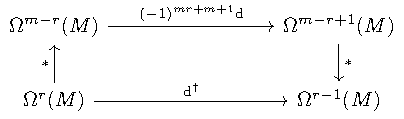
\includegraphics{figures/riemannian geometry/commutative/fig.pdf}
        \end{center}
\begin{theorem}
    Let $(M,g)$ be a compact orientable manifold without a boundary and $\alpha\in\Omega^r(M)$, $\beta\in\Omega^{r-1}(M)$.
    Then
    \begin{align}
        (\md \beta,\alpha)=(\beta,\md^\dagger \alpha).
    \end{align}
\end{theorem}
\begin{proof}
    Recall that $\dd(\beta\wedge\ast\alpha)=\dd{\beta}\wedge\ast\alpha-(-1)^r \beta\wedge\dd{\ast\alpha}$.
    Suppose $(M,g)$ is Riemannian.
    Noting that $\dd{\ast\alpha}$ is an $(m-r+1)$-form and $(-1)^{(m-r+1)[m-(m-r+1)]}\ast\ast=(-1)^{mr+m+r+1}\ast\ast$ is an identity map.
    \begin{align}\label{eq:adjointderivativeinner}
        \dd(\beta\wedge\ast\alpha)=\dd{\beta}\wedge\ast\alpha-(-1)^{mr+m+1}\beta\wedge\ast(\ast\dd{\ast\alpha}).
    \end{align}
    Integrating \eqref{eq:adjointderivativeinner} over $M$, we have 
    \begin{align}
        \int_M\dd{\beta}\wedge\ast\alpha-\int_M \beta\wedge\ast[(-1)^{mr+m+1}\ast\dd{\ast\alpha}]=\int_M\dd(\beta\wedge\ast\alpha)=\int_{\partial M}\beta\wedge\ast\alpha=0
    \end{align}
    where we have assumed that integration on the boundary vanishes.
    This shows $(\dd{\beta},\alpha)=(\beta,\md^\dagger\alpha)$.

    The Lorentzian case can be proved in the same way.
\end{proof}


\subsubsection{The Laplacian, Harmonic Forms and the Hodge Decomposition Theorem}
\begin{definition}[Laplacian]
    The \textbf{Laplacian} $\Delta:\Omega^r(M)\to\Omega^r(M)$ is defined by
    \begin{align}
        \Delta\equiv(\md+\md^\dagger)^2=\md\md^\dagger+\md^\dagger\md.
    \end{align}
\end{definition}
\begin{example}[Explicit form of $\Delta:\Omega^0(M)\to\Omega^0(M)$]
    Let $f\in\mathcal{F}(M)$.
    Since $\md^\dagger f=0$, we have
    \begin{align}
        \Delta f= & \md^\dagger\md f=-\ast\md\ast\left(\partial_\mu f\dd{x^\mu}\right)\notag                                                                                                                       \\
        =         & -\ast\dd(\frac{\sqrt{\abs{g}}}{(m-1)!}\partial_\mu fg^{\mu\nu}\epsilon_{\lambda\nu_2\dots\nu_m}\dd{x^{\nu_2}}\wedge\dots\wedge\dd{x^{\nu_m}})\notag                                            \\
        =         & -\ast\frac{1}{(m-1)!}\partial_\nu\left[\sqrt{\abs{g}}g^{\lambda\mu}\partial_\mu f\right]\epsilon_{\lambda\nu_2\dots\nu_m}\dd{x^\nu}\wedge\dd{x^{\nu_2}}\wedge\dots\wedge\dd{x^{\nu_m}}\notag   \\
        =         & -\ast\frac{1}{(m-1)!}\sum_{\nu}\partial_\nu\left[\sqrt{\abs{g}}g^{\nu\mu}\partial_\mu f\right]\epsilon_{\nu\nu_2\dots\nu_m}\dd{x^\nu}\wedge\dd{x^{\nu_2}}\wedge\dots\wedge\dd{x^{\nu_m}}\notag \\
        =         & -\ast\partial_\nu\left[\sqrt{\abs{g}}g^{\nu\mu}\partial_\mu f\right]\dd{x^1}\wedge\dd{x^{2}}\wedge\dots\wedge\dd{x^{m}}\notag                                                                  \\
        =         & \partial_\nu\left[\sqrt{\abs{g}}g^{\nu\mu}\partial_\mu f\right]\sqrt{\abs{g}}\epsilon^{12\dots m}\notag                                                                                        \\
        =         & \partial_\nu\left[\sqrt{\abs{g}}g^{\nu\mu}\partial_\mu f\right]\sqrt{\abs{g}}g^{-1}\notag                                                                                                      \\
        =         & -\frac{1}{\sqrt{\abs{g}}}\partial_\nu\left[\sqrt{\abs{g}}g^{\nu\mu}\partial_\mu f\right].
    \end{align}
\end{example}
\begin{property}
    Let $(M,g)$ be a compact Riemannian manifold.
    The Laplacian $\Delta$ is a positive positive operator on $M$:
    \begin{align}
        (\omega,\Delta\omega)=(\omega,(\md^\dagger\md+\md\md^\dagger)\omega)=(\dd{\omega},\dd{\omega})+(\md^\dagger\omega,\md^\dagger\omega)\geq0.
    \end{align}
\end{property}

\begin{definition}[Harmonic, closed and coclosed forms]
    An $r$-form is called
    \begin{itemize}
        \item \textbf{harmonic} if $\Delta\omega=0$
        \item \textbf{closed} if $\dd{\omega}=0$
        \item \textbf{coclosed} if $\md^\dagger\omega=0$.
    \end{itemize}
\end{definition}
\begin{theorem}\label{closedandcoclosed}
    An $r$-form $\omega$ is harmonic if and only if $\omega$ is closed and coclosed.
\end{theorem}
\begin{proof}
    If $\omega$ is harmonic, then
    \begin{align}
        0=(\omega,\Delta\omega)=(\omega,(\md^\dagger\md+\md\md^\dagger)\omega)=(\dd{\omega},\dd{\omega})+(\md^\dagger\omega,\md^\dagger\omega)\geq0
    \end{align}
    which implies $\dd{\omega}=0$ and $\md^\dagger\omega=0$.
\end{proof}
\begin{definition}[Coexact forms]
    An $r$-form $\omega$ is called \textbf{coexact} if it is written \textit{globally} as
    \begin{align}
        \omega_r=\md^\dagger\beta_{r+1},
    \end{align}
    where $\beta_{r+1}\in\Omega^{r+1}(M)$.
\end{definition}

We denote the set of harmonic $r$-forms on $M$ by $\mathrm{Harm}^r(M)$ and the set of exact $r$-forms (coexact $r$-forms) by $\dd{\Omega^{r-1}(M)}$ ($\md^\dagger\Omega^{r+1}(M)$).
\begin{theorem}[Hodge decomposition theorem]\label{Hodgedecompositiontheorem}
    Let $(M,g)$ be a compact orientable Riemannian manifold without boundary.
    Then $\Omega^r(M)$ is uniquely decomposed as
    \begin{align}
        \Omega^r(M)=\dd{\alpha_{r-1}}+\md^\dagger\beta_{r+1}+\gamma_r,\label{eq:Hodgedecomposition}
    \end{align}
    where $\dd{\alpha_{r-1}}\in\dd{\Omega^{r-1}(M)}$, $\md^\dagger\beta_{r+1}\in\md^\dagger\Omega^{r+1}(M)$ and $\gamma_r\in\mathrm{Harm}^r(M)$.
    \eqref{eq:Hodgedecomposition} can be also written as
    \begin{align}
        \Omega^r(M)=\dd{\Omega^{r-1}(M)}\oplus\md^\dagger\Omega^{r+1}(M)\oplus\mathrm{Harm}^r(M).
    \end{align}

    If $r=0$, we define $\Omega^{-1}(M)\equiv\{0\}$.
\end{theorem}
Before proving \cref{Hodgedecompositiontheorem}, we need three lemmas.
\begin{lemma}
    Follow the notation of \cref{Hodgedecompositiontheorem},
    \begin{align}
        (\dd{\alpha_{r-1}},\md^\dagger\beta_{r+1})=(\dd{\alpha_{r-1}},\gamma_r)=(\md^\dagger\beta_{r+1},\gamma_r)=0.
    \end{align}
    and if $\omega_{r}\in\Omega^r(M)$ satisfies
    \begin{align}
        (\dd{\alpha_{r-1}},\omega_r)=(\md^\dagger\beta_{r+1},\omega_r)=(\gamma_r,\omega_r)=0
    \end{align}
    for any $\dd{\alpha_{r-1}}\in\dd{\Omega^{r-1}(M)}$, $\md^\dagger\beta_{r+1}\in\md^\dagger\Omega^{r+1}(M)$ and $\gamma_r\in\mathrm{Harm}^r(M)$, then $\omega_r=0$.
\end{lemma}
\begin{proof}
    The proof is straightforward:
    \begin{align}
        (\dd{\alpha_{r-1}},\md^\dagger\beta_{r+1}) & =(\md^2\alpha_{r-1},\beta_{r+1})=0    \\
        (\dd{\alpha_{r-1},\gamma_r})               & =(\alpha_{r-1},\md^\dagger\gamma_r)=0 \\
        (\md^\dagger\beta_{r+1},\gamma_r)          & =(\beta_{r+1},\dd{\gamma_r})=0
    \end{align}
    where we have used \cref{closedandcoclosed}.
    
    If $\forall\alpha_{r-1}\in\Omega^{r-1}(M)$ we have $(\dd{\alpha_{r-1}},\omega_r)=0$, then just let $\alpha_{r-1}=\md^\dagger\omega_r$
    \begin{align}
        (\dd(\md^\dagger\omega_r),\omega_r)=(\md^\dagger\omega_r,\md^\dagger\omega_r)=0
    \end{align}
    which means $\md^\dagger\omega_r=0$.
    In the same way, we can choose $\beta_{r+1}=\dd{\omega_r}$ and we have $\dd{\omega_r}=0$.
    So $\Delta\omega_r=0$ and we can choose $\gamma_r=\omega_r$ and get $(\omega_r,\omega_r)=0$ which means $\omega_r=0$.
\end{proof}
\begin{lemma}\label{lemma:harmonicorthogonal}
    If $\omega_r\in\Omega^r(M)$ is written as $\omega_r=\Delta\psi_r$ for some $\psi_r\in\Omega^r(M)$, then $(\omega_r,\gamma_r)=0$ for any $\gamma_r\in\mathrm{Harm}^r (M)$.
\end{lemma}
\begin{proof}
    Recall that $\Delta\equiv\md^\dagger\md+\md\md^\dagger$ and notice that $\Delta\gamma_r=0$, we have
    \begin{align}
        (\omega_r,\gamma_r)=(\Delta\psi_r,\gamma_r)=(\psi_r,\Delta\gamma_r)=0.
    \end{align}
\end{proof}
\begin{lemma}\label{lemma:converseharmonicorthogonal}
    If $\omega_r\in\Omega^r(M)$ is orthogonal to any harmonic $r$-form, then $\omega_r$ is written as $\Delta\psi_r$ for some $\psi_r\in\Omega^r(M)$
\end{lemma}
\Cref{lemma:converseharmonicorthogonal} is the converse of \cref{lemma:harmonicorthogonal} and it is also true but the proof is higly technical.
We only need to know that the operator $\Delta^{-1}$ (the Green function) is well defined in the current context and $\psi_r$ is given by $\Delta^{-1}\omega_r$.
\paragraph{Proof of \cref{Hodgedecompositiontheorem}}
We are now ready to prove \cref{Hodgedecompositiontheorem}
\begin{proof}
    Let $P:\Omega^r(M)\to\mathrm{Harm}^r(M)$ be a projection operator to the space of harmonic $r$-forms\snm.
    Take an element $\omega_r\in\Omega^r(M)$.
    It can be proved that $\omega_r-P\omega_r$ is orthogonal\snm to $\mathrm{Harm}^r(M)$, so it can be written as $\Delta\psi_r$ for some $\psi_r\in\Omega^r(M)$.
    Then we have
    \begin{align}
        \omega_r=\dd(\md^\dagger\psi_r)+\md^\dagger(\dd{\psi_r})+P\omega_r\label{eq:hodgedecompositionrealization}
    \end{align}
    which realizes the decomposition of \cref{Hodgedecompositiontheorem}.
\end{proof}
\snt{$\mathrm{Harm}^r(M)$ is a subspace of $\Omega^r(M)$ and according to the conclusions of linear algebra, there is a unique decomposition of a differential form into a harmonic part and a non-harmonic part. $P$ is the map from a differential form to its harmonic part.}
\snt{If $C$ is a closed vector subspace of a Hilbert space $H$ then $H=C\oplus C^{\perp}$.}


\subsubsection{Harmonic Forms and de Rham Cohomology Groups}
\begin{theorem}[Hodge's theorem]\label{theorem:Hodgestheorem}
    On a compact orientable Riemannian manifold $(M,g)$, $H^r(M)$ is isomorphic to $\mathrm{Harm}^r(M)$:
    \begin{align}
        H^r(M)\cong\mathrm{Harm}^r(M).
    \end{align}
    The isomorphism is provided by identifying $[\omega]\in H^r(M)$ with $P\omega\in\mathrm{Harm}^r(M)$.
\end{theorem}
We need two lemmas to prove \cref{theorem:Hodgestheorem}.
\begin{lemma}\label{lemma:Hodgestheorem1}
    Any element of the de Rham cohomology group has a unique harmonic representative which implies\snm $H^r(M)\subset\mathrm{Harm}^r(M)$.
\end{lemma}
\snt{Be careful about the abuse of notation here. $H^r(M)\subset\mathrm{Harm}^r(M)$ here actually means $H^r(M)$ can be mapped into a subset of $\mathrm{Harm}^r(M)$.}
\begin{proof}
    Let $[\omega_r]\in H^r(M)$.
    Using \cref{Hodgedecompositiontheorem}, $\omega_r$ is decomposed as $\omega_r=\gamma_r+\dd{\alpha_{r-1}}+\md^\dagger\beta_{r+1}$.
    Since $\dd{\omega_r}=0$, we have
    \begin{align}
        0=(\dd{\omega_r},\beta_{r+1})=(\md\md^\dagger\beta_{r+1},\beta_{r+1})=(\md^\dagger\beta_{r+1},\md^\dagger\beta_{r+1}),
    \end{align}
    which implies $\md^\dagger\beta_{r+1}=0$ and $\omega_r=\gamma_r+\dd{\alpha_{r-1}}$.
    So $\omega_r\in\mathrm{Harm}^r(M)\oplus\dd{\Omega^{r-1}(M)}$.
    From \eqref{eq:hodgedecompositionrealization} we have
    \begin{align}
        \omega_r=P\omega_r+\dd(\md^\dagger\psi)=P\omega_r+\md\md^\dagger\Delta^{-1}\omega_r.
    \end{align}
    $\gamma_r\equiv P\omega_r$ is the harmonic representative of $[\omega_r]$.

    Let $\widetilde{\omega}_r$ be another representative of $[\omega_r]$: $\widetilde{\omega}_r-\omega_r=\dd{\eta_{r-1}}$, $\eta_{r-1}\in\Omega^{r-1}(M)$.
    We have
    \begin{align}
        \widetilde{\omega}_r=P\widetilde{\omega}_r+\dd(\md^\dagger\Delta^{-1}\widetilde{\omega}_r)=P\omega_r+\dd(\md^\dagger\Delta^{-1}\widetilde{\omega}_r),
    \end{align}
    where the last equality follows since $\dd{\eta_{r-1}}$ is orthogonal to $\mathrm{Harm}^r(M)$.
    So $[\omega_r]$ has a unique harmonic representative $P\omega_r$.
\end{proof}
\begin{lemma}\label{lemma:Hodgestheorem2}
    $H^r(M)\supset\mathrm{Harm}^r(M)$.
\end{lemma}
\begin{proof}
    $Z^r(M)\supset\mathrm{Harm}^r(M)$ since $\forall\gamma_r\in\mathrm{Harm}^r(M)$, $\dd{\gamma_r}=0$.
    
    We also have $B^r(M)\cap\mathrm{Harm}^r(M)=\emptyset$ since $B^r(M)=\dd{\Omega^{r-1}(M)}$ from \eqref{eq:Hodgedecomposition}.
    
    Thus, each element in $\mathrm{Harm}^r(M)$ belongs to a different element in $H^r(M)$ and hence $\mathrm{Harm}^r(M)\subset H^r(M)$.
\end{proof}
\paragraph{Proof of \cref{theorem:Hodgestheorem}} We can now easily prove \cref{theorem:Hodgestheorem}
\begin{proof}
    Combine \cref{lemma:Hodgestheorem1,lemma:Hodgestheorem2}, \cref{theorem:Hodgestheorem} is directly proved.
\end{proof}
\begin{property}
    From \cref{theorem:Hodgestheorem}, we have 
    \begin{align}
        \dim\mathrm{Harm}^r(M)=\dim H^r(M)=b^r
    \end{align}
    where $b^r$ is the Betti number.
    The Euler characteristic is given by 
    \begin{align}
        \chi(M)=\sum(-1)^r b^r=\sum(-1)^r\dim\mathrm{Harm}^r(M).\label{eq:eulerharm}
    \end{align}
    The LHS of \eqref{eq:eulerharm} is a topological quantity while the RHS is an analytical quantity given by the eigenvalue problem of the Laplacian $\Delta$. 
\end{property}

\subsection{Aspects of General Relativity}
\subsubsection{Introduction to General Relativity}
Einstein proposed the following principles to construct the general theory of relativity
\begin{itemize}
    \item \textbf{General Principle of Relativity}: All laws in physics take the same forms in any coordinate system.
    \item \textbf{Principle of Equivalence}: The trajectory of a point mass in a gravitational field depends only on its initial position and velocity, and is independent of its composition and structure.
          And there exists a coordinate system in which the effect of a gravitational field vanishes locally.
\end{itemize}
\begin{remark}
    The general principle of relativity has a more mathematical form called \textit{general covariance}, which states that Local laws of physics are the same in all coordinate systems.
    General covariance is applied by expressing laws using tensors.

    The principle of equivalence tells us that the motion of an free small object in independent of itself and only depend on the geometry of the spacetime, which implies we can use metric to describe spacetime.
    The principle of equivalence also means that on a Lorentzian manifold $M$ we can always find coordinates in the neighbourhood of $p\in M$ such that
    \begin{align}
        g_{\mu\nu}(p)=\eta_{\mu\nu}\qand g_{\mu\nu,\rho}(p)=0.
    \end{align}
    These are exactly the normal coordinates system we discussed before in \cref{normalcoordinates}.
\end{remark}

Any theory of gravity must reduce to Newton's theory of gravity in the weak-field limit.
In Newton's theory, the gravitational potential $\Phi$ satisfies the Poisson equation
\begin{align}\label{nequation}
    \Delta\Phi=4\pi G\rho,
\end{align}
where $\rho$ is the mass density and $\Delta$ is the Laplace operator.

In general relativity, the gravitational potential is replaced by the components of the metric tensor.
Then, instead of the LHS of \cref{nequation}, we have the \textbf{Einstein tensor} defined by
\begin{align}
    G_{\mu\nu}\equiv Ric_{\mu\nu}-\frac{1}{2}g_{\mu\nu}\mathcal{R}
\end{align}
Similarly, the mass density is replaced by a more general object called the \textbf{energy-momentum tensor} $T_{\mu\nu}$.
\lec{Einstein equation}{}And the \textbf{Einstein equation} is \sidenote{The constant $8\pi G$ is chosen so that \cref{einsteinequation} reproduces the Newtonian result in the weak-field limit.}
\begin{align}\label{einsteinequation}
    G_{\mu\nu}=8\pi GT_{\mu\nu}.
\end{align}
\begin{remark}
    The tensor $T_{\mu\nu}$ is obtained from the matter action by the variational principle.
    From Noether's theorem, $T_{\mu\nu}$ must satisfy a conservation equation of the form $\nabla_{\mu}T^{\mu\nu}=0$.
\end{remark}

\subsubsection{Einstein-Hilbert Action}
We define the \textbf{Einstein-Hilbert action} by
\begin{align}
    S_{\text{EH}}\equiv\frac{1}{16\pi G}\int\mathcal{R}\sqrt{-g}\dd[4]{x}.
\end{align}
\begin{proposition}
    Let $(M,g)$ be a (pseudo-)Riemannian manifold.
    Under the variation $g_{\mu\nu}\to g_{\mu\nu}+\delta g_{\mu\nu}$ , $g^{\mu\nu}$, $g$ and $Ric_{\mu\nu}$ changes as
    \begin{itemize}
        \item $\delta g^{\mu\nu}=-g^{\mu\kappa}g^{\lambda\nu}\delta g_{\kappa\lambda}$
        \item $\delta g=gg^{\mu\nu}\delta g_{\mu\nu}\qc \delta\sqrt{\abs{g}}=\frac{1}{2}\sqrt{\abs{g}}g^{\mu\nu}\delta g_{\mu\nu}$
        \item $\delta Ric_{\mu\nu}=\nabla_{\kappa}\delta\tensor{\Gamma}{^\kappa_\nu_\mu}-\nabla_\nu\delta\tensor{\Gamma}{^\kappa_\kappa_\mu}$\quad(\textbf{Palatini identity}).
    \end{itemize}
\end{proposition}
\begin{proof}
    to be added
\end{proof}

Suppose there exists matter described by an action
\begin{align}
    S_{\text{M}}\equiv\int\mathcal{L}(\phi)\sqrt{-g}\dd[4]{x}
\end{align}
where $\mathcal{L}(\phi)$ is the Lagrangian density of the theory.
\begin{example}
    The Lagrangian of the real scalar field and the electromagnetic field are
    \begin{align}
        S_{\text{S}}  & \equiv-\frac{1}{2}\left[g^{\mu\nu}\partial_\mu\phi\partial_\nu\phi+m^2\phi^2\right]\sqrt{-g}\dd[4]{x} \\
        S_{\text{EM}} & \equiv-\frac{1}{4}\int F_{\mu\nu}F^{\mu\nu}\sqrt{-g}\dd[4]{x}
    \end{align}
    where $F_{\mu\nu}=\partial_\mu A_\nu-\partial_\nu A_\mu=\nabla_\mu A_\nu-\nabla_\nu A_\mu$.
\end{example}

\subsubsection{Spinors in Curved Spacetime}
\begin{intu}
    Quantum field theory should be locally and covariantly constructed\cite{Hollands:2014eia}.
\end{intu}
Consider a Dirac spinor $\psi$ in a 4-dimensional Lorentz manifold $M$.
The vierbein $\tensor{\tilde{e}}{^\alpha_\mu}$ defined by
\begin{align}
    g_{\mu\nu}\equiv \tensor{\tilde{e}}{^\alpha_\mu}\tensor{\tilde{e}}{^\beta_\nu}\eta_{\alpha\beta}
\end{align}
defines an orthonormal frame $\{\hat{\theta}^\alpha=\tensor{\tilde{e}}{^\alpha_\mu}\dd{x^\mu}\}$ at each point $p\in M$.
With respect to this frame, we define
\begin{align}
    \hat{\gamma}^\alpha\equiv\tensor{\tilde{e}}{^\alpha_\mu}\gamma^\mu
\end{align}
where $\gamma^\mu$ are Dirac matrices, and $\hat{\gamma}^\alpha$ satisfy
\begin{align}
    \acomm{\hat{\gamma}^\alpha}{\hat{\gamma}^\beta}=2\eta^{\alpha\beta}.
\end{align}

Under a local Lorentz transformation $\tensor{\Lambda}{^\alpha_\beta}(p)$, the Dirac spinor transforms as
\begin{align}
    \psi(p)\to\rho(\Lambda)\psi(p)\quad \bar{\psi}(p)\to\bar{\psi}(p)\rho(\Lambda)^{-1}
\end{align}
where $\bar{\psi}\equiv\psi^\dagger\gamma^0$ and $\rho(\Lambda)$ is the spinor representation of $\Lambda$.

\paragraph{Construction of Lagrangian}
To construct an invariant action, we seek a covariant derivative $\tilde{\nabla}_\alpha \psi (\alpha=0,1,2,3)$ that transforms under local Lorentz transformation $\Lambda$ as
\begin{align}
    \tilde{\nabla}_\alpha\psi\to\rho(\Lambda)\tensor{\Lambda}{_\alpha^\beta}\tilde{\nabla}_\beta\psi.\label{seekcovariant}
\end{align}
And the invariant Lagrangian will look like
\begin{align}
    \mathcal{L}=\bar{\psi}(\ii\hat{\gamma}^\alpha\tilde{\nabla}_\alpha+m)\psi
\end{align}
Notice that $\tensor{\tilde{e}}{_\alpha^\mu}\partial_\mu\psi$ transforms under $\Lambda(p)$ as\sidenote{The Lorentz transformation here will change the vierbein and thus also change the component of Dirac spinors or 4-vectors.}
\begin{align}
    \tensor{\tilde{e}}{_\alpha^\mu}\partial_\mu\psi\to\tensor{\Lambda}{_\alpha^\beta}\tensor{\tilde{e}}{_\beta^\mu}\partial_\mu\rho(\Lambda)\psi=\tensor{\Lambda}{_\alpha^\beta}\tensor{e}{_\beta^\mu}[\rho(\Lambda)\partial_\mu\psi+\partial_\mu\rho(\Lambda)\psi].\label{epartialpsi}
\end{align}
We use the ansatz
\begin{align}
    \tilde{\nabla}_\alpha\psi=\tensor{\tilde{e}}{_\alpha^\mu}[\partial_\mu+\Omega_\mu]\psi.
\end{align}
From \eqref{seekcovariant} and \eqref{epartialpsi}, $\Omega_\mu$ satisfies
\begin{align}
    \Omega_\mu\to\rho(\Lambda)\Omega_\mu\rho(\Lambda)^{-1}-\partial_\mu\rho(\Lambda)\rho(\Lambda)^{-1}.\label{omegamu}
\end{align}
Consider an infinitesimal local Lorentz transformation $\tensor{\Lambda}{_\alpha^\beta}(p)=\tensor{\delta}{_\alpha^\beta}+\tensor{\epsilon}{_\alpha^\beta}(p)$.
The Dirac spinor transforms as
\begin{align}
    \psi\to\exp(\frac{1}{2}\ii\epsilon^{\alpha\beta}\Sigma_{\alpha\beta})\approx\left(1+\frac{1}{2}\ii\epsilon^{\alpha\beta}\Sigma_{\alpha\beta}\right)\psi
\end{align}
where $\Sigma_{\alpha\beta}\equiv\frac{1}{4}\ii\acomm{\hat{\gamma}_\alpha}{\hat{\gamma}_\beta}$ is the spinor representation of the generators of the Lorentz transformation.
$\Sigma_{\alpha\beta}$ satisfies the O(1,3) Lie algebra
\begin{align}
    i\comm{\Sigma_{\alpha\beta}}{\Sigma_{\gamma\delta}}=\eta_{\gamma\beta}\Sigma_{\alpha\delta}-\eta_{\gamma\alpha}\Sigma_{\beta\delta}+\eta_{\delta\beta}\Sigma_{\gamma\alpha}-\eta_{\delta\alpha}\Sigma_{\gamma\delta}.\label{spinorliealgebra}
\end{align}
Under the same Lorentz transformation, $\Omega_\mu$ transforms as
\begin{align}
    \Omega_\mu\to & \left(1+\frac{1}{2}\ii\epsilon^{\alpha\beta}\Sigma_{\alpha\beta}\right)\Omega_\mu\left(1-\frac{1}{2}\ii\epsilon^{\gamma\delta}\Sigma_{\gamma\delta}\right)-\frac{1}{2}\ii\partial_\mu \epsilon^{\alpha\beta}\Sigma_{\alpha\beta}\left(1-\frac{1}{2}\ii\epsilon^{\gamma\delta}\Sigma_{\gamma\delta}\right)\notag \\
    =             & \Omega_\mu+\frac{1}{2}\epsilon^{\alpha\beta}\comm{\Sigma_{\alpha\beta}}{\Omega_\mu}-\frac{1}{2}\ii\partial_\mu\epsilon^{\alpha\beta}\Sigma_{\alpha\beta}+\order{\epsilon^2}\label{omegamutrans}
\end{align}
and keep only the first order term.
Notice that $\tensor{\omega}{^\alpha_\beta}$ transforms under an infinitesimal Lorentz transformation as
\begin{align}
    \tensor{\omega}{^\alpha_\beta}\to\tensor{\omega}{^\alpha_\beta}+\tensor{\epsilon}{^\alpha_\gamma}\tensor{\omega}{^\gamma_\beta}-\tensor{\omega}{^\alpha_\gamma}\tensor{\epsilon}{^\gamma_\beta}-\dd{\tensor{\epsilon}{^\alpha_\beta}}
\end{align}
or in components
\begin{align}
    \tensor{\Gamma}{^\alpha_\mu_\beta}\to\tensor{\Gamma}{^\alpha_\mu_\beta}+\tensor{\epsilon}{^\alpha_\gamma}\tensor{\Gamma}{^\gamma_\mu_\beta}-\tensor{\Gamma}{^\alpha_\mu_\gamma}\tensor{\epsilon}{^\gamma_\beta}-\partial_\mu\tensor{\epsilon}{^\alpha_\beta}.
\end{align}
With all these above, we can prove that the combination
\begin{align}
    \Omega_\mu\equiv\frac{1}{2}\ii\tensor{\Gamma}{^\alpha_\mu^\beta}\Sigma_{\alpha\beta}=\frac{1}{2}\ii\tensor{\tilde{e}}{^\alpha_\nu}\nabla_\nu \tilde{e}^{\beta\nu}\Sigma_{\alpha\beta}\label{cnlorentz}
\end{align}
satisfies the transformation property \eqref{omegamu}:
\begin{proof}
    Using \eqref{spinorliealgebra} \eqref{omegamutrans} and \eqref{cnlorentz}, we have
    \begin{align}
        \frac{1}{2}\ii\tensor{\Gamma}{^\alpha_\mu^\beta}\Sigma_{\alpha\beta}
    \end{align}
\end{proof}


\subsection{Bosonic String Theory}

\subsubsection{The String Action}

The action of a relativistic particle is the length of the world line
\begin{align}
    S\equiv m\int_{s_{\text{i}}}^{s_{\text{f}}}\dd{s}=m\int_{\tau_{\text{i}}}^{\tau_{\text{f}}}\dd{\tau}\left(-\dot{X}^\mu \dot{X}_\mu\right)^{\frac{1}{2}}
\end{align}
where $\dot{X}^\mu\equiv\dd{X}^\mu/\dd{\tau}$.
It is often convenient to take another expression,
\begin{align}
    S\equiv-\frac{1}{2}\int\dd{\tau}\sqrt{g}\left(g^{-1}\dot{X}^\mu\dot{X}_\mu-m^2\right),
\end{align}
where the auxiliary variable $g\equiv g_{\tau\tau}$ is regarded as a metric.

Nambu proposed \textbf{Nambu action}, an action describing the strings, which is proportional to the area of the world sheet, the surface spanned by the trajectory of a string
\begin{align}
    S=-\frac{1}{2\pi\alpha'}\int_{0}^{\pi}\dd{\sigma}\int_{\tau_{\text{i}}}^{\tau_{\text{f}}}\dd{\tau}\left[-\det\left(\partial_\alpha X^\mu \partial_\beta X_\mu\right)\right]
\end{align}
where $\xi^0=\tau$, $\tau^1=\sigma$ and $\partial_\alpha X^\mu\equiv\partial X^\mu/\partial\xi^\alpha$.

A quadratic action for strings is called the \textbf{Polyakov action} and is given by
\begin{align}\label{Polyakov}
    S=-\frac{1}{4\pi\alpha'}\int_{0}^\pi\dd{\sigma}\int^{\tau_{\text{f}}}_{\tau_{\text{i}}}\dd{\tau}\sqrt{-g}g^{\alpha\beta}\partial_\alpha X^\mu \partial_\beta X_\mu
\end{align}
where $g=\det g_{\alpha\beta}$ and $g^{\alpha\beta}=\left(g^{-1}\right)^{\alpha\beta}$.
\paragraph{Equation of motion} 
Our variational parameters are $X^\mu$ and $g_{\alpha\beta}$.

Under the variation of $\delta X^\mu$, we have 
\begin{align}
    \partial_\alpha\left(\sqrt{-g}g^{\alpha\beta}\partial_\beta X_\mu\right)=0
\end{align}

Under the variation of $\delta g_{\alpha\beta}$, we have 
\begin{align}
    \partial_\alpha X^\mu \partial_\beta X_\mu-\frac{1}{2}g_{\alpha\beta}\left(g^{\lambda\delta}\partial_\gamma X^\mu\partial_\delta X_\mu\right)=0\label{eq:stringmetric}
\end{align}
and \eqref{eq:stringmetric} gives 
\begin{align}
    g_{\alpha\beta}=\partial_\alpha X^\mu \partial_\beta X^\nu \eta_{\mu\nu}\label{eq:stringmetricinduced}
\end{align}
which shows the induced metric agrees with $g_{\alpha\beta}$.
Substitute \eqref{eq:stringmetricinduced} back into \eqref{Polyakov} to eliminate $g_{\alpha\beta}$, we will recover the Nambu action.

\subsubsection{Symmetries of the Polyakov Strings}
We assume the physical spacetime is Minkowskian $(\rr^D,\eta)$.
The bosonic string theory is defined on a two-dimensional Lorentz manifold $(M,g)$.
The embedding $f:M\to\rr^D$ is defined by $\xi^\alpha\mapsto X^\mu$ where $\{\xi^\alpha\}=(\tau,\sigma)$ are the local coordinates of $M$.

The Polyakov action
\begin{align}
    S=-\frac{1}{2}\int\dd[2]{\xi}\sqrt{-g}g^{\alpha\beta}\partial_a X^\mu\partial_\beta X^\nu\eta_{\mu\nu}\label{eq:Polyakov2}
\end{align} 
is invariant under
\begin{itemize}
    \item local reparametrization $\mathrm{Diff}(M)$ of the world sheet
          \begin{align}
              \tau\to\tau'(\tau,\sigma)\quad\sigma\to\sigma'(\tau,\sigma)
          \end{align}
          since the volume element $\sqrt{-g}\dd[2]{\xi}$ is invariant and $g^{\alpha\beta}\partial_\alpha X^\mu\partial_\beta X_\mu$ is a scalar.
    \item global Poincar\'e invariance
          \begin{align}
              X^\mu\to {X^{\mu}}'\equiv\tensor{\Lambda}{^\mu_\nu}X^\nu+a^\mu \quad\Lambda\in\text{SO}(D-1,1)\quad a\in\mathbb{R}^D.\label{eq:stringpoincare}
          \end{align}
          Under \eqref{eq:stringpoincare}, the action \eqref{eq:Polyakov2} transforms as 
          \begin{align}
            S\to S'=&-\frac{1}{2}\int\dd[2]{\xi}\sqrt{-g}g^{\alpha\beta}\partial_\alpha\left(\tensor{\Lambda}{^\mu_\kappa}X^\kappa+a^\mu\right)\partial_\beta\left(\tensor{\Lambda}{^\nu_\lambda}X^\lambda+a^\nu\right)\eta_{\mu\nu}\notag\\
                =&-\frac{1}{2}\int\dd[2]{\xi}\sqrt{-g}g^{\alpha\beta}\partial_\alpha X^\kappa\partial_\beta X^\lambda\left(\tensor{\lambda}{^\mu_\kappa}\tensor{\Lambda}{^\nu_\lambda}\eta_{\mu\nu}\right)\notag\\
                =&-\frac{1}{2}\int\dd[2]{\xi}\sqrt{-g}g^{\alpha\beta}\partial_\alpha X^\kappa\partial_\beta X^\lambda=S.
          \end{align}
    \item Weyl rescaling
          \begin{align}
              g_{\alpha\beta}\to g'_{\alpha\beta}\equiv\me^{\phi(\sigma,\tau)}g_{\alpha\beta}.\label{eq:stringweyl}
          \end{align}
          Under \eqref{eq:stringweyl}, the action \eqref{eq:Polyakov2} transforms as 
          \begin{align}
            S\to S'=&-\frac{1}{2}\int\dd[2]{\xi}\sqrt{-\me^{4\sigma}g}\me^{-2\sigma}g^{\alpha\beta}\partial_\alpha X^\mu\partial_\beta X^\nu \eta_{\mu\nu}\notag\\
                =&-\frac{1}{2}\int\dd[2]{\xi}\sqrt{-g}g^{\alpha\beta}\partial_\alpha X^\kappa\partial_\beta X^\lambda=S.
          \end{align}
          Note that the Weyl rescaling invariance exists only when $M$ is two dimensional, making strings prominent among other extended objccts such as membranes.
\end{itemize}
\begin{remark}
    Since $\dim M=2$, we can always parametrize the world sheet by the isothermal coordinate so that
    \begin{align}
        g_{\alpha\beta}=\me^{2\sigma(\tau,\sigma)}\eta_{\alpha\beta}.
    \end{align}
    Then the Weyl rescaling invariance allows us to choose the standard metric $\eta_{\alpha\beta}$ on the world sheet.

    The metric $g_{\alpha\beta}$ has three independent components while the reparametrization has two degrees of freedom and the Weyl scaling invariance has one.
    Thus, so long as we are dealing with strings, we can choose the standard metric $\eta_{\alpha\beta}$.
\end{remark}
\clearpage

\section{Complex Manifolds}
\begin{intu}
    A complex manifold admits a complex structure in which each coordinate neighbourhood is homeomorphic to $\mathbb{C}^m$ and the transition from one coordinate system to the other is analytic.
\end{intu}

\subsection{Complex Manifolds}
\begin{definition}[Holomorphic function]
    A complex-valued function $f:\mathbb{C}^m\to\mathbb{C}$ is \textbf{holomorphic} if $f=f_1+\ii f_2$ satisfies the \textbf{Cauchy-Riemann relations} for each argument $z^\mu=x^\mu+\ii y^\mu$,
    \begin{align}
        \pdv{f_1}{x^\mu}=\pdv{f_2}{y^\mu}\quad\pdv{f_2}{x^\mu}=-\pdv{f_1}{y^\mu}.
    \end{align}
\end{definition}
A map $(f^1,\dots,f^n):\mathbb{C}^m\to\mathbb{C}^n$ is called holomorphic if each function $f^\lambda\ (1\leq\lambda\leq n)$ is holomorphic.
\subsubsection{Definitions}
\begin{definition}[Complex manifold]
    $M$ is a \textbf{complex manifold} if :
    \begin{enumerate}
        \item $M$ is a topological space 
        \item $M$ is provided with a family of pairs $\{(U_i,\phi_i)\}$
        \item $\{U_i\}$ is a family of open sets which covers $M$.
              The map $\phi_i$ is a homeomorphism from $U_i$ to an open subset $U$ of $\mathbb{C}^m$.\snm
        \item Given $U_i$ and $U_j$ such that $U_i\cap U_j\neq\emptyset$, the map $\psi_{ji}\equiv\phi_j\circ\phi_i^{-1}$ from $\phi_i(U_i\cap U_j)$ to $\phi_j(U_i\cap U_j)$ is holomorphic.
    \end{enumerate}
\end{definition}
\snt{Hence $M$ is even dimensional.}
The number $m$ is called the \textit{complex dimension} of $M$ and is denoted as $\dim_{\mathbb{C}}=m$.
The real dimension $2m$ is denoted by $\dim_\mathbb{R} M$ or simply $\dim M$.

\subsubsection{Examples}
\subsection{Calculus on Complex Manifolds}
\subsubsection{Holomorphic Maps}
\subsubsection{Complexifications}
\subsubsection{Almost Complex Structure}
\subsection{Complex Differential Forms}
\subsubsection{Complexification of Real Differential Forms}

\clearpage
\section{Fibre Bundles}



\clearpage
\bibliographystyle{jhep}
\bibliography{ref}


\clearpage
\listoftheorems[ignoreall,title={List of Definitions}, onlynamed={definition}, swapnumber]

\end{document}